\documentclass[12pt,a4paper]{report}

% ======================== PAKET ========================
\usepackage[indonesian]{babel}
\usepackage[utf8]{inputenc}
\usepackage[T1]{fontenc}
\usepackage{geometry}
\usepackage{graphicx}
\usepackage{hyperref}
\usepackage{xcolor}
\usepackage{caption}
\usepackage{subcaption}
\usepackage{booktabs}
\usepackage{longtable}
\usepackage{array}
\usepackage{tabularx}
\usepackage{enumitem}
\usepackage{fancyhdr}
\usepackage{titlesec}
\usepackage{float}
\usepackage{amsmath}
\usepackage{amsfonts}
\usepackage{amssymb}
\usepackage{setspace}
\usepackage{parskip}

% ======================== GEOMETRI ========================
\geometry{top=3cm, bottom=3cm, left=4cm, right=3cm}

% ======================== WARNA TEMA (DESIGN.md) ========================
\definecolor{primarygreen}{HTML}{84BD3A}   % Primary Green
\definecolor{tealdark}{HTML}{32735F}       % Teal Dark
\definecolor{midnight}{HTML}{0B2B40}       % Midnight Blue
\definecolor{gold}{HTML}{FEBE0D}           % Gold
\definecolor{linen}{HTML}{F9FAF7}          % Linen
\definecolor{sage}{HTML}{DEE2DE}           % Sage
\definecolor{iron}{HTML}{6B7280}           % Iron
\definecolor{obsidian}{HTML}{171717}       % Obsidian

% ======================== HYPERREF ========================
\hypersetup{
    colorlinks=true,
    linkcolor=midnight,
    urlcolor=tealdark,
    citecolor=tealdark,
    pdftitle={Panduan Operasional dan Manajemen Situs Web Profil Kelurahan Salomallori},
    pdfauthor={A. Muh Muflih Hanifatussurur - KKN Universitas Hasanuddin},
    pdfsubject={Buku Panduan Website Profil Kelurahan Salomallori}
}

% ======================== JUDUL SEKSI ========================
\titleformat{\chapter}[display]
  {\normalfont\huge\bfseries\color{midnight}}
  {\chaptertitlename\ \thechapter}
  {20pt}
  {\Huge}
\titlespacing*{\chapter}{0pt}{-30pt}{20pt}

\titleformat{\section}
  {\normalfont\Large\bfseries\color{tealdark}}
  {\thesection}{1em}{}
\titleformat{\subsection}
  {\normalfont\large\bfseries\color{obsidian}}
  {\thesubsection}{1em}{}
\titleformat{\subsubsection}
  {\normalfont\normalsize\bfseries\color{obsidian}}
  {\thesubsubsection}{1em}{}

% ======================== HEADER & FOOTER ========================
\pagestyle{fancy}
\setlength{\headheight}{24.02pt}
\addtolength{\topmargin}{-12.02pt}
\fancyhf{}
\fancyhead[L]{\small\color{midnight}\textbf{Kelurahan Salomallori}}
\fancyhead[R]{\small\color{iron}Panduan Operasional Situs Web}
\fancyfoot[C]{\thepage}
\renewcommand{\headrulewidth}{0.4pt}
\renewcommand{\headrule}{\hbox to\headwidth{\color{midnight}\leaders\hrule height \headrulewidth\hfill}}

% ======================== CAPTION ========================
\captionsetup{font=small, labelfont={bf,color=tealdark}, justification=centering}

% ======================== JUDUL BAB/BAGIAN NON-NOMOR ========================
\newcommand{\unnumberedchapter}[1]{%
  \chapter*{#1}%
  \addcontentsline{toc}{chapter}{#1}%
}

% ======================== DOKUMEN ========================
\begin{document}

% ============================================================
% COVER / HALAMAN UTAMA
% ============================================================
\begin{titlepage}
\begin{center}

\vspace*{1cm}

{\color{midnight}\rule{\linewidth}{3pt}}\\[0.5cm]
{\color{gold}\rule{\linewidth}{1pt}}\\[1.2cm]

{\fontsize{20pt}{26pt}\selectfont\bfseries\color{midnight}
PANDUAN OPERASIONAL DAN MANAJEMEN\\ SITUS WEB PROFIL\\ KELURAHAN SALOMALLORI
}\\[0.8cm]

{\color{gold}\rule{0.4\linewidth}{1.5pt}}\\[0.8cm]

{\large\color{obsidian}
Petunjuk Teknis Integrasi Informasi Kelurahan,\\ Etalase Produk UMKM, Dokumentasi Kegiatan,\\ dan Pemeliharaan Data Statistik Visual
}\\[1.2cm]

{\color{midnight}\rule{\linewidth}{1pt}}\\[0.3cm]
{\color{midnight}\rule{\linewidth}{3pt}}\\[1.5cm]

\begin{tabular}{ll}
\textbf{Target Pengguna} & : Masyarakat Umum (Warga Kelurahan \& Pengunjung) \\
                        & \quad \& Pengelola Sistem (Perangkat Kelurahan, Administrator, \& Editor) \\
\textbf{Alamat Domain}   & : \url{https://www.salomallori.web.id} \\
\end{tabular}

\vfill

{\large\textbf{Disusun Oleh:}}\\
{\normalsize A. Muh Muflih Hanifatussurur (H071231062 -- Sistem Informasi)}\\
{\normalsize Tim Kuliah Kerja Nyata (KKN) Universitas Hasanuddin}\\
{\normalsize Kelurahan Salomallori}\\[0.5cm]

{\Large\textbf{2026}}

\end{center}
\end{titlepage}

% ============================================================
% BAGIAN AWAL
% ============================================================

% ---------- KATA PENGANTAR ----------
\unnumberedchapter{KATA PENGANTAR}

Assalamu'alaikum Warahmatullahi Wabarakatuh.

Puji dan syukur kami panjatkan ke hadirat Tuhan Yang Maha Esa karena atas rahmat dan karunia-Nya, buku panduan berjudul \emph{Panduan Operasional dan Manajemen Situs Web Profil Kelurahan Salomallori} ini dapat diselesaikan dengan baik.

Buku panduan ini disusun sebagai bagian dari program kerja Tim Kuliah Kerja Nyata (KKN) Universitas Hasanuddin di Kelurahan Salomallori, Kecamatan Dua Pitue, Kabupaten Sidenreng Rappang. Kehadiran buku ini diharapkan menjadi jembatan penghubung antara teknologi digital dengan kebutuhan informasi masyarakat, sehingga seluruh potensi kelurahan -- baik dari segi profil kewilayahan, potensi UMKM, dokumentasi kegiatan, maupun data statistik -- dapat dikelola dan disajikan secara transparan, terpadu, dan berkelanjutan.

Buku ini ditujukan bagi dua kelompok pengguna utama, yaitu masyarakat umum sebagai pengguna layanan informasi publik dan perangkat kelurahan sebagai pengelola sistem. Untuk itu, penyusunan materi dibagi ke dalam enam bab yang mencakup pendahuluan, dasar teori dan arsitektur sistem, persyaratan sistem, langkah-langkah penggunaan dan pengelolaan, studi kasus, serta penutup. Setiap bab disusun dengan bahasa yang sederhana agar mudah dipahami oleh seluruh kalangan, baik yang memiliki latar belakang teknis maupun tidak.

Kami mengucapkan terima kasih yang sebesar-besarnya kepada Lurah Salomallori beserta seluruh perangkat kelurahan, warga masyarakat, dosen pembimbing, serta semua pihak yang telah memberikan dukungan, masukan, dan partisipasi aktif sehingga website profil kelurahan beserta buku panduan ini dapat terwujud.

Akhir kata, kami menyadari bahwa buku panduan ini masih jauh dari sempurna. Oleh karena itu, kritik dan saran yang membangun sangat kami harapkan demi perbaikan di masa mendatang. Semoga buku panduan ini memberikan manfaat bagi kelurahan dan seluruh masyarakat.

Wassalamu'alaikum Warahmatullahi Wabarakatuh.

\vspace{1.5cm}
\begin{flushright}
Salomallori, 2026\\
Tim KKN Universitas Hasanuddin\\
Kelurahan Salomallori
\end{flushright}

% ---------- DAFTAR ISI ----------
\tableofcontents
\clearpage

% ---------- DAFTAR GAMBAR ----------
\listoffigures
\clearpage

% ---------- DAFTAR TABEL ----------
\listoftables
\clearpage

% ============================================================
% BAB 1: PENDAHULUAN
% ============================================================
\chapter{PENDAHULUAN}

\section{Latar Belakang}

Kelurahan Salomallori merupakan salah satu kelurahan yang berada di Kecamatan Dua Pitue, Kabupaten Sidenreng Rappang (Sidrap), Provinsi Sulawesi Selatan. Kelurahan ini memiliki luas wilayah sebesar \textbf{7,63 km²} dengan jumlah penduduk sebanyak \textbf{3.234 jiwa}. Seluruh penduduk tersebut tergabung dalam \textbf{1.077 kepala keluarga (KK)} yang tersebar di \textbf{3 lingkungan}.

Secara administratif, Kelurahan Salomallori memiliki batas-batas wilayah sebagai berikut:
\begin{enumerate}[leftmargin=2em, itemsep=2pt]
    \item Sebelah \textbf{Utara} berbatasan dengan Desa Ajubissue (Kecamatan Pitu Riawa);
    \item Sebelah \textbf{Timur} berbatasan dengan Kelurahan Tanrutedong;
    \item Sebelah \textbf{Selatan} berbatasan dengan Desa Kampale;
    \item Sebelah \textbf{Barat} berbatasan dengan Desa Padangloang Alau.
\end{enumerate}

Kelurahan Salomallori memiliki potensi utama yang meliputi sektor \emph{pertanian padi sawah}, \emph{peternakan ayam ras petelur}, serta \emph{kerajinan dan kuliner lokal}. Potensi-potensi tersebut selama ini belum terpublikasikan secara luas dan terintegrasi dalam satu wadah digital yang mudah diakses oleh masyarakat umum, calon investor, maupun pemangku kepentingan lainnya.

Perkembangan teknologi informasi yang pesat menuntut setiap institusi, termasuk pemerintah kelurahan, untuk menghadirkan layanan informasi yang transparan dan mudah diakses. Kehadiran media digital menjadi sangat penting untuk:
\begin{enumerate}[leftmargin=2em, itemsep=2pt]
    \item Mempromosikan potensi kelurahan kepada khalayak yang lebih luas;
    \item Memperkenalkan produk-produk UMKM lokal kepada calon pembeli dan investor;
    \item Menyediakan informasi publik yang transparan mengenai profil, kegiatan, dan data statistik kelurahan.
\end{enumerate}

Berdasarkan kebutuhan tersebut, Tim KKN Universitas Hasanuddin membangun \textbf{Website Profil Kelurahan Salomallori} yang dapat diakses melalui domain resmi \url{https://www.salomallori.web.id}. Website ini dirancang sebagai portal informasi terpadu yang memadukan profil kelurahan, kabar desa, katalog UMKM, galeri foto, dan visualisasi data statistik dalam satu platform yang modern, responsif, dan mudah dikelola.

\section{Tujuan Pedoman}

Buku panduan ini disusun dengan tujuan sebagai berikut:
\begin{enumerate}[leftmargin=2em, itemsep=2pt]
    \item Menyediakan panduan teknis penggunaan fitur publik bagi warga kelurahan dan pengunjung untuk menjelajahi informasi digital terpadu Kelurahan Salomallori;
    \item Menyediakan panduan operasional bagi perangkat kelurahan dalam mengelola dan menyebarkan informasi publik melalui dashboard administrator dan editor;
    \item Menjamin keberlanjutan tata kelola platform digital kelurahan pasca-kegiatan KKN Universitas Hasanuddin.
\end{enumerate}

\section{Sasaran Pengguna}

Buku panduan ini ditujukan kepada tiga kelompok sasaran utama, yaitu:
\begin{enumerate}[leftmargin=2em, itemsep=2pt]
    \item \textbf{Masyarakat Umum / Warga Kelurahan / Investor}, yaitu pengguna layanan informasi publik yang menjelajahi konten website seperti profil kelurahan, berita, UMKM, galeri, dan infografis;
    \item \textbf{Perangkat Kelurahan (Administrator \& Editor)}, yaitu pengelola sistem yang bertanggung jawab memperbarui dan memelihara konten website;
    \item \textbf{Tim KKN Universitas Hasanuddin}, yaitu pengembang yang akan melakukan serah terima sistem dan menjadi narasumber dalam pelatihan penggunaan website.
\end{enumerate}

% ============================================================
% BAB 2: DASAR TEORI & ARSITEKTUR SISTEM
% ============================================================
\chapter{DASAR TEORI \& ARSITEKTUR SISTEM}

\section{Pengertian \& Gambaran Umum Platform}

Website Profil Kelurahan Salomallori adalah portal informasi digital resmi yang dibangun menggunakan arsitektur web modern. Secara teknis, sistem dibangun dengan teknologi sebagai berikut:
\begin{enumerate}[leftmargin=2em, itemsep=2pt]
    \item \textbf{Next.js 16 (App Router)} sebagai framework utama pengembangan aplikasi;
    \item \textbf{React 19} sebagai pustaka antarmuka pengguna (UI library);
    \item \textbf{Tailwind CSS 4} sebagai kerangka kerja CSS untuk desain yang responsif;
    \item \textbf{PostgreSQL} sebagai sistem manajemen basis data;
    \item \textbf{Prisma ORM} sebagai penghubung aplikasi dengan basis data;
    \item \textbf{Better-Auth} untuk sistem autentikasi dan otorisasi;
    \item \textbf{TipTap} sebagai editor teks kaya (\emph{rich text editor});
    \item \textbf{Cloudinary} untuk pengelolaan dan unggahan media gambar.
\end{enumerate}

Desain visual website menerapkan gaya \emph{Editorial-First}, \emph{Minimalism}, dan \emph{Glassmorphism} dengan navigasi mengapung (\emph{floating architecture}). Palet warna resmi yang digunakan mengacu pada \emph{Design System} Kelurahan Salomallori, yaitu \textbf{Primary Green} \textcolor{primarygreen}{\textbf{\#84BD3A}}, \textbf{Teal Dark} \textcolor{tealdark}{\textbf{\#32735F}}, \textbf{Midnight Blue} \textcolor{midnight}{\textbf{\#0B2B40}}, dan \textbf{Gold} \textcolor{gold}{\textbf{\#FEBE0D}}, dengan tipografi Montserrat untuk judul serta Geist untuk teks isi.

\begin{figure}[H]
    \centering
    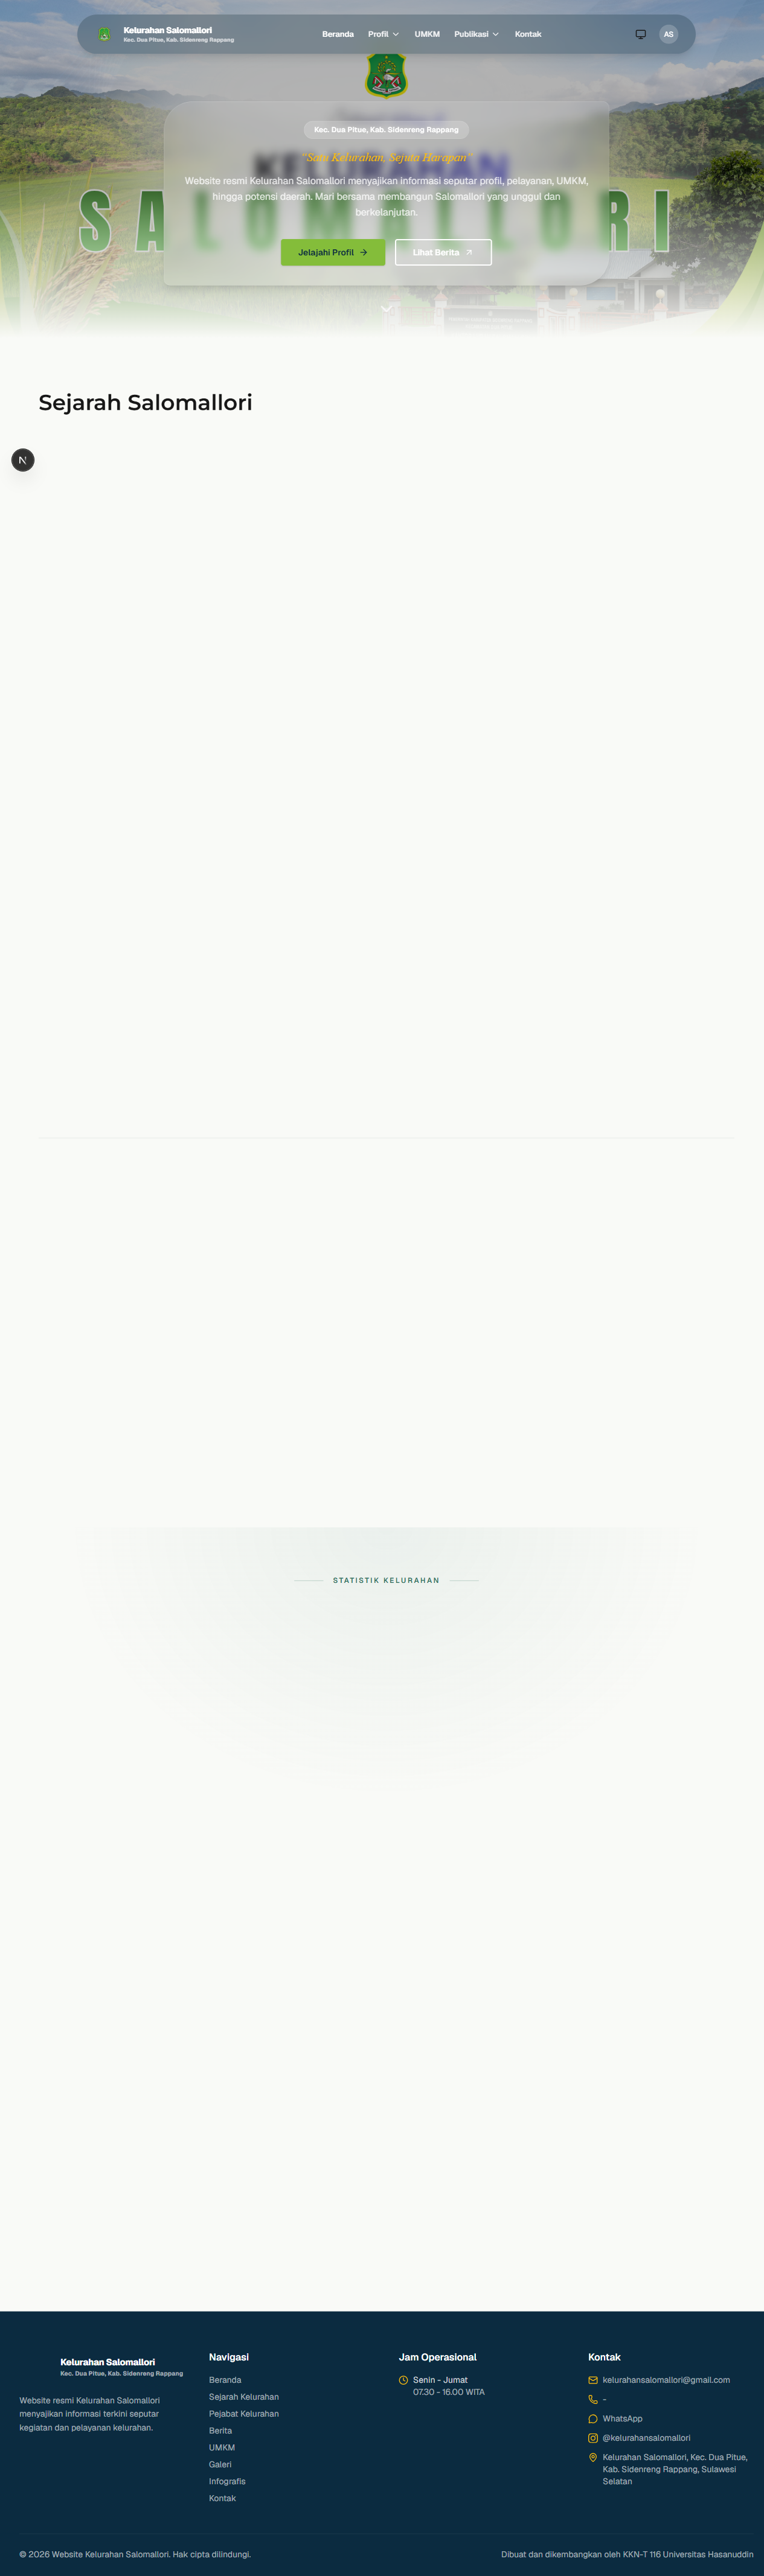
\includegraphics[width=0.85\textwidth]{images/beranda.png}
    \caption{Tampilan Beranda Website Profil Kelurahan Salomallori}
    \label{fig:beranda}
\end{figure}

\section{Komponen Utama Website Profil Kelurahan}

Website Profil Kelurahan Salomallori terdiri atas beberapa komponen utama sebagai berikut:
\begin{enumerate}[leftmargin=2em, itemsep=2pt]
    \item \textbf{Profil Kelurahan}, mencakup Sejarah Kelurahan, Pejabat Kelurahan, dan Infografis statistik demografi;
    \item \textbf{Kabar Desa}, yaitu berita terkini seputar kegiatan dan informasi kelurahan;
    \item \textbf{Katalog Potensi (UMKM Lokal)}, yaitu etalase produk usaha mikro, kecil, dan menengah warga;
    \item \textbf{Galeri Foto Digital (Potret Desa)}, yaitu dokumentasi kegiatan dan keindahan kelurahan;
    \item \textbf{Kontak Kelurahan \& Jam Operasional}, yaitu informasi alamat, telepon, WhatsApp, email, dan peta lokasi.
\end{enumerate}

\section{Pembagian Hak Akses Pengguna (\emph{Role-Based Access Control} / RBAC)}

Sistem menggunakan autentikasi \textbf{Better-Auth} untuk mengelola pembagian hak akses pengguna. Terdapat tiga level pengguna dengan kewenangan yang berbeda, sebagaimana ditunjukkan pada Tabel~\ref{tab:rbac}.

\begin{table}[H]
    \centering
    \caption{Matriks Pembagian Hak Akses Pengguna}
    \label{tab:rbac}
    \begin{tabular}{lccc}
        \toprule
        \textbf{Fitur / Kemampuan} & \textbf{USER} & \textbf{EDITOR} & \textbf{ADMIN} \\
        \midrule
        Menjelajahi konten publik & \checkmark & \checkmark & \checkmark \\
        Mengirim pesan / kontak kelurahan & \checkmark & \checkmark & \checkmark \\
        Mengelola berita (Post) & --- & \checkmark & \checkmark \\
        Mengelola UMKM & --- & \checkmark & \checkmark \\
        Mengelola galeri foto & --- & \checkmark & \checkmark \\
        Mengelola profil kelurahan & --- & --- & \checkmark \\
        Mengelola infografis & --- & --- & \checkmark \\
        Mengelola kontak \& pesan masuk & --- & --- & \checkmark \\
        Mengelola pengguna & --- & --- & \checkmark \\
        \bottomrule
    \end{tabular}
\end{table}

Keterangan peran:
\begin{enumerate}[leftmargin=2em, itemsep=2pt]
    \item \textbf{USER (Warga)}: pengguna umum yang dapat melihat seluruh konten publik dan mengirim pesan;
    \item \textbf{EDITOR (Perangkat Kelurahan)}: pengelola konten yang dapat menambah dan mengubah berita, UMKM, serta galeri foto;
    \item \textbf{ADMIN (Super Admin)}: pengelola penuh yang memiliki seluruh akses termasuk pengaturan profil kelurahan, infografis, kontak, pesan masuk, dan manajemen pengguna.
\end{enumerate}

% ============================================================
% BAB 3: PERSYARATAN & KEBUTUHAN SISTEM
% ============================================================
\chapter{PERSYARATAN \& KEBUTUHAN SISTEM}

\section{Kebutuhan Perangkat Pengguna Umum (Warga Kelurahan \& Pengunjung)}

Masyarakat umum yang ingin mengakses Website Profil Kelurahan Salomallori tidak memerlukan perangkat khusus. Persyaratan yang dibutuhkan cukup sederhana sebagaimana ditunjukkan pada Tabel~\ref{tab:req-user}.

\begin{table}[H]
    \centering
    \caption{Kebutuhan Perangkat Pengguna Umum}
    \label{tab:req-user}
    \begin{tabularx}{\textwidth}{llX}
        \toprule
        \textbf{Komponen} & \textbf{Spesifikasi} & \textbf{Keterangan} \\
        \midrule
        Perangkat & Smartphone, Tablet, atau Laptop & Sistem dirancang responsif sehingga tampil optimal di semua ukuran layar \\
        Browser & Google Chrome, Mozilla Firefox, Microsoft Edge, Safari & Versi terbaru yang mendukung standar web modern \\
        Koneksi Internet & Stabil & Diperlukan untuk memuat konten, gambar, dan peta \\
        Akun & Tidak wajib & Akses konten publik dapat dilakukan tanpa login \\
        \bottomrule
    \end{tabularx}
\end{table}

\section{Kebutuhan Perangkat Pengelola (Administrator \& Editor Kelurahan)}

Perangkat kelurahan yang bertindak sebagai Administrator atau Editor membutuhkan perangkat dan akses yang sedikit lebih lengkap, sebagaimana ditunjukkan pada Tabel~\ref{tab:req-admin}.

\begin{table}[H]
    \centering
    \caption{Kebutuhan Perangkat Pengelola (Administrator \& Editor)}
    \label{tab:req-admin}
    \begin{tabularx}{\textwidth}{llX}
        \toprule
        \textbf{Komponen} & \textbf{Spesifikasi} & \textbf{Keterangan} \\
        \midrule
        Perangkat & PC atau Laptop Admin & Disarankan layar minimal 13 inci untuk kenyamanan mengelola dashboard \\
        Browser & Google Chrome atau Microsoft Edge (versi terbaru) & Untuk mengakses halaman dashboard \\
        Akun Login & Terotentikasi (USER / EDITOR / ADMIN) & Difasilitasi oleh sistem Better-Auth \\
        Koneksi Internet & Stabil & Diperlukan saat menyimpan konten dan mengunggah media ke Cloudinary \\
        \bottomrule
    \end{tabularx}
\end{table}

\section{Alur Akses Platform}

Terdapat tiga alur akses utama dalam platform, yaitu:

\subsection{Alur Akses Publik}

Pengguna umum mengakses seluruh fitur publik melalui menu navigasi utama yang meliputi:
\begin{enumerate}[leftmargin=2em, itemsep=2pt]
    \item \textbf{Beranda} (Halaman utama);
    \item \textbf{Profil} (\emph{dropdown}: Sejarah Kelurahan, Pejabat Kelurahan, Infografis);
    \item \textbf{UMKM} (Katalog produk lokal);
    \item \textbf{Publikasi} (\emph{dropdown}: Berita, Galeri Foto);
    \item \textbf{Kontak} (Informasi kontak dan peta lokasi).
\end{enumerate}

\subsection{Alur Dashboard Warga}

Pengguna warga yang telah terdaftar dapat mengakses halaman profil pribadinya melalui alamat \texttt{/akun/[id]}. Halaman ini menampilkan informasi profil akun masing-masing pengguna.

\subsection{Alur Dashboard Administrator \& Editor}

Administrator dan Editor mengelola seluruh konten melalui halaman \texttt{/dashboard} beserta sub-menu yang tersedia. Akses ke dashboard dilakukan melalui halaman login terlebih dahulu.

\begin{figure}[H]
    \centering
    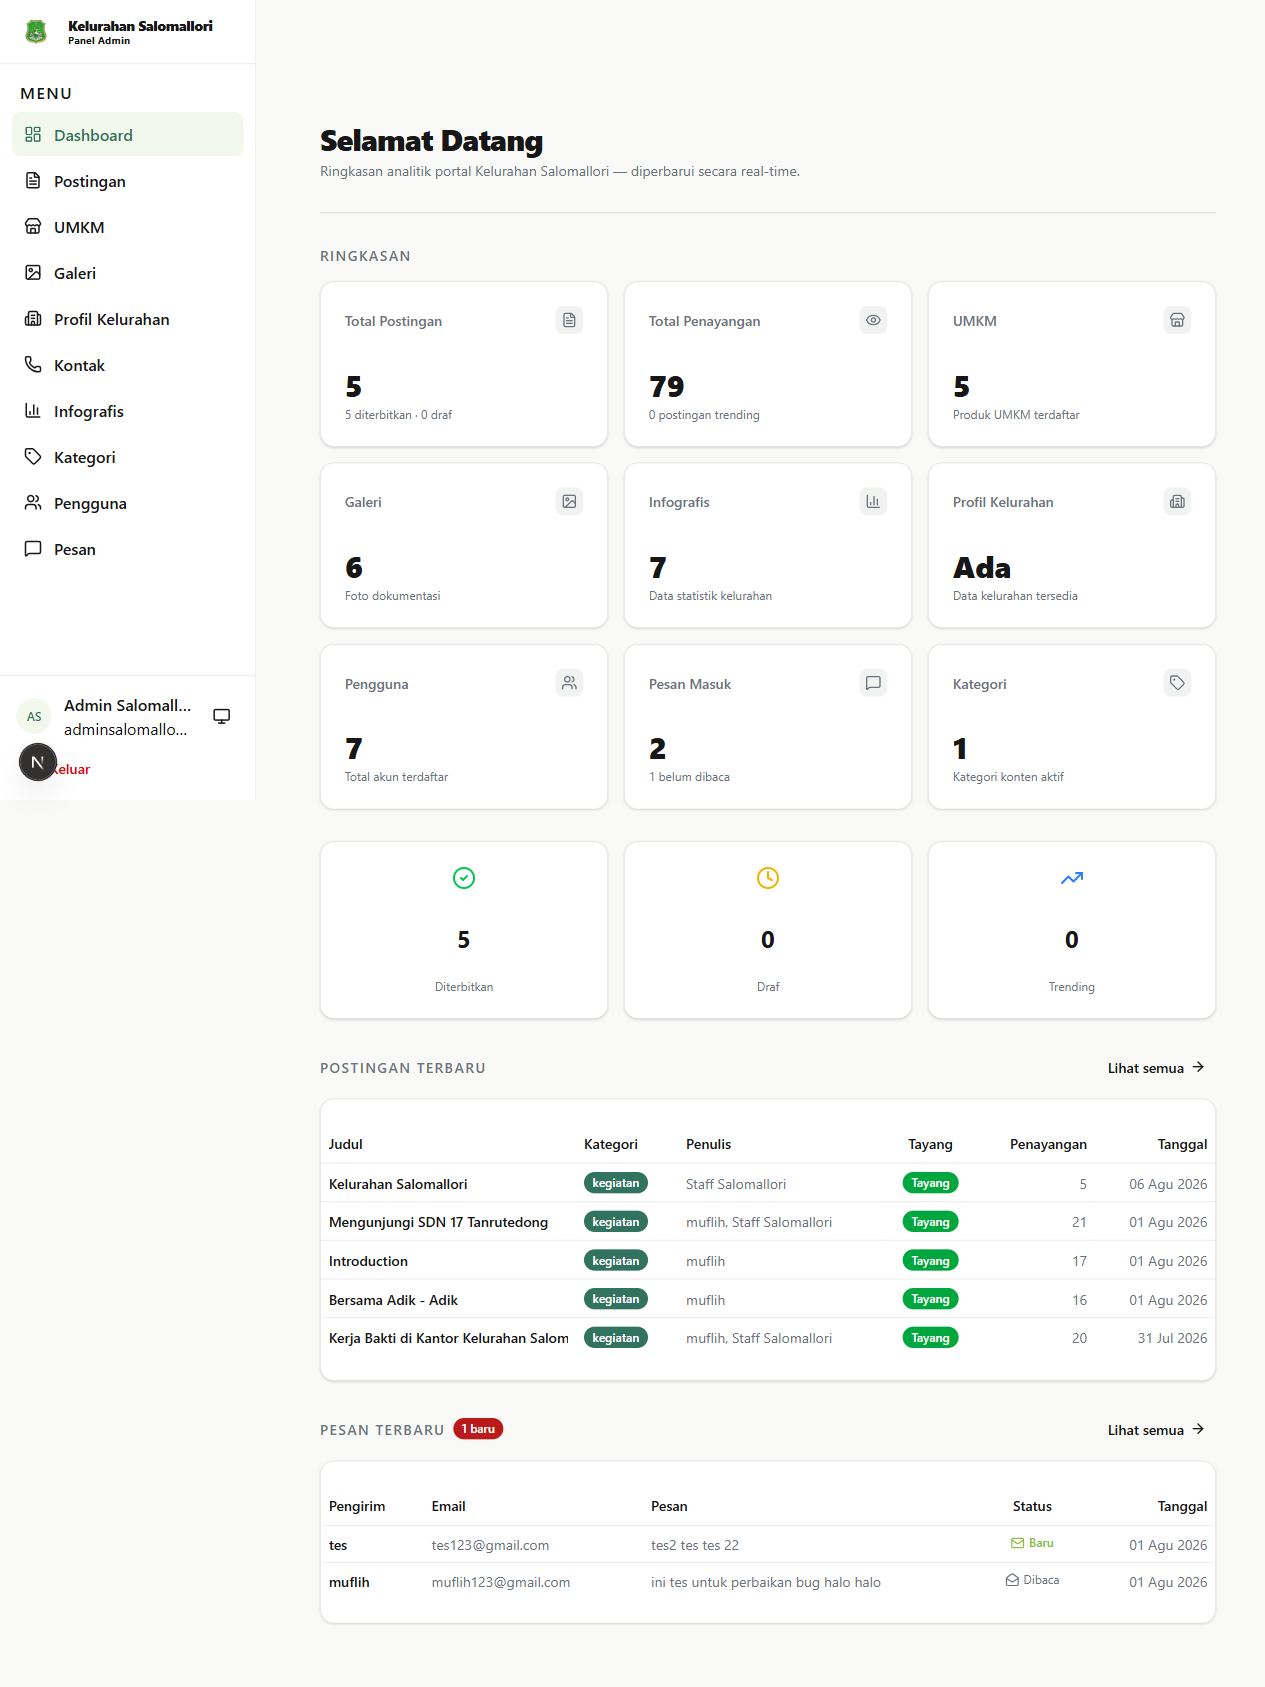
\includegraphics[width=0.7\textwidth]{images/login.png}
    \caption{Halaman Masuk (Login) Administrator dan Editor}
    \label{fig:login}
\end{figure}

% ============================================================
% BAB 4: LANGKAH-LANGKAH PENGGUNAAN DAN PENGELOLAAN
% ============================================================
\chapter{LANGKAH-LANGKAH PENGGUNAAN DAN PENGELOLAAN}

\section{Panduan Pengguna Umum (Masyarakat \& Pengunjung)}

\subsection{Membuka Halaman Utama \& Navigasi \emph{Floating Pill}}

Langkah-langkah membuka halaman utama:
\begin{enumerate}[leftmargin=2em, itemsep=2pt]
    \item Buka peramban (browser) pada perangkat yang digunakan;
    \item Ketik alamat domain resmi \url{https://www.salomallori.web.id} pada kolom alamat;
    \item Halaman Beranda akan tampil dengan navigasi utama berbentuk \emph{floating pill} di bagian atas yang berisi menu \textbf{Beranda}, \textbf{Profil}, \textbf{UMKM}, \textbf{Publikasi}, dan \textbf{Kontak};
    \item Pada halaman Beranda, pengunjung dapat melihat ringkasan data kelurahan yang meliputi luas wilayah, jumlah jiwa, jumlah KK, dan jumlah lingkungan secara langsung.
\end{enumerate}

\begin{figure}[H]
    \centering
    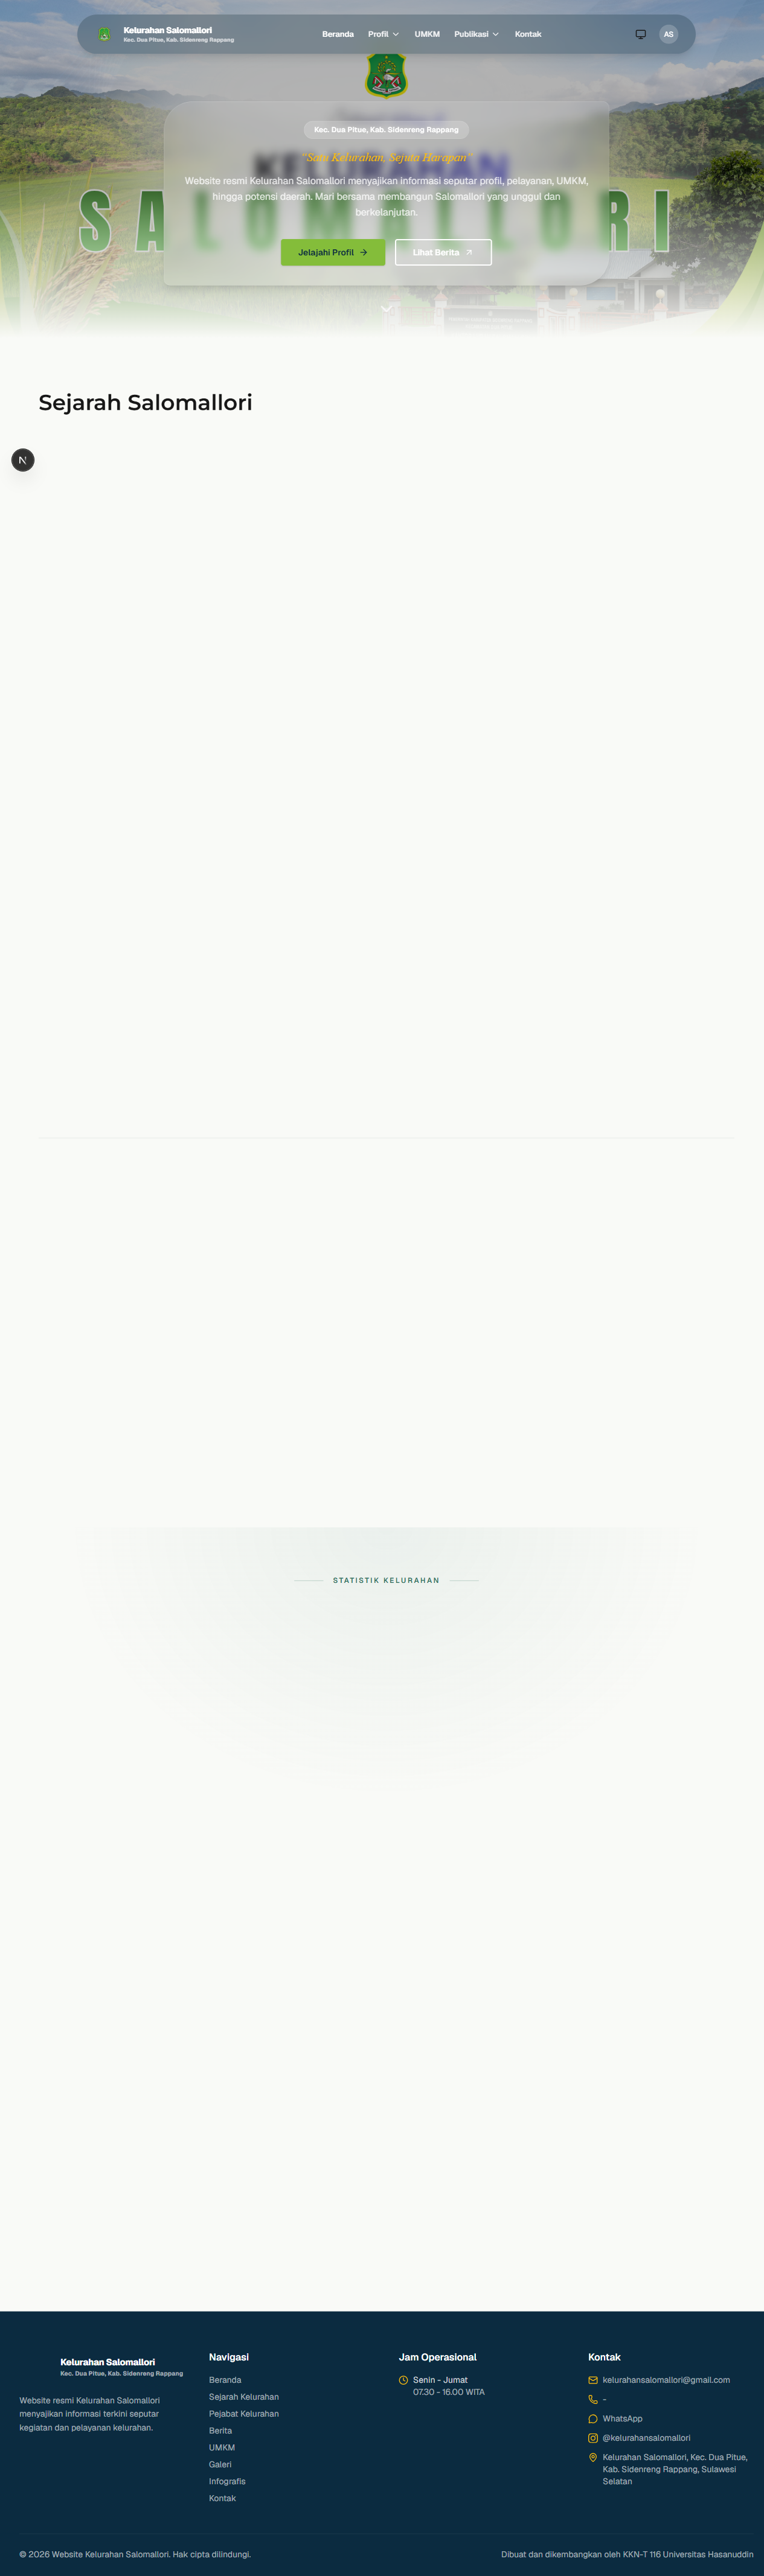
\includegraphics[width=0.85\textwidth]{images/beranda.png}
    \caption{Ringkasan Data Kelurahan pada Halaman Beranda}
    \label{fig:beranda-stats}
\end{figure}

\subsection{Menjelajahi Menu Profil (Sejarah, Pejabat, \& Infografis)}

Langkah-langkah menjelajahi menu Profil:
\begin{enumerate}[leftmargin=2em, itemsep=2pt]
    \item Arahkan kursor ke menu \textbf{Profil} pada navigasi utama;
    \item Muncul \emph{dropdown} yang berisi sub-menu \textbf{Sejarah Kelurahan}, \textbf{Pejabat Kelurahan}, dan \textbf{Infografis};
    \item Pilih \textbf{Sejarah Kelurahan} untuk membaca sejarah kelurahan lengkap dengan data batas wilayah;
    \item Pilih \textbf{Pejabat Kelurahan} untuk melihat daftar pejabat dan perangkat kelurahan beserta fotonya;
    \item Pilih \textbf{Infografis} untuk mengeksplorasi visualisasi data statistik kelurahan.
\end{enumerate}

\begin{figure}[H]
    \centering
    \begin{subfigure}{0.45\textwidth}
        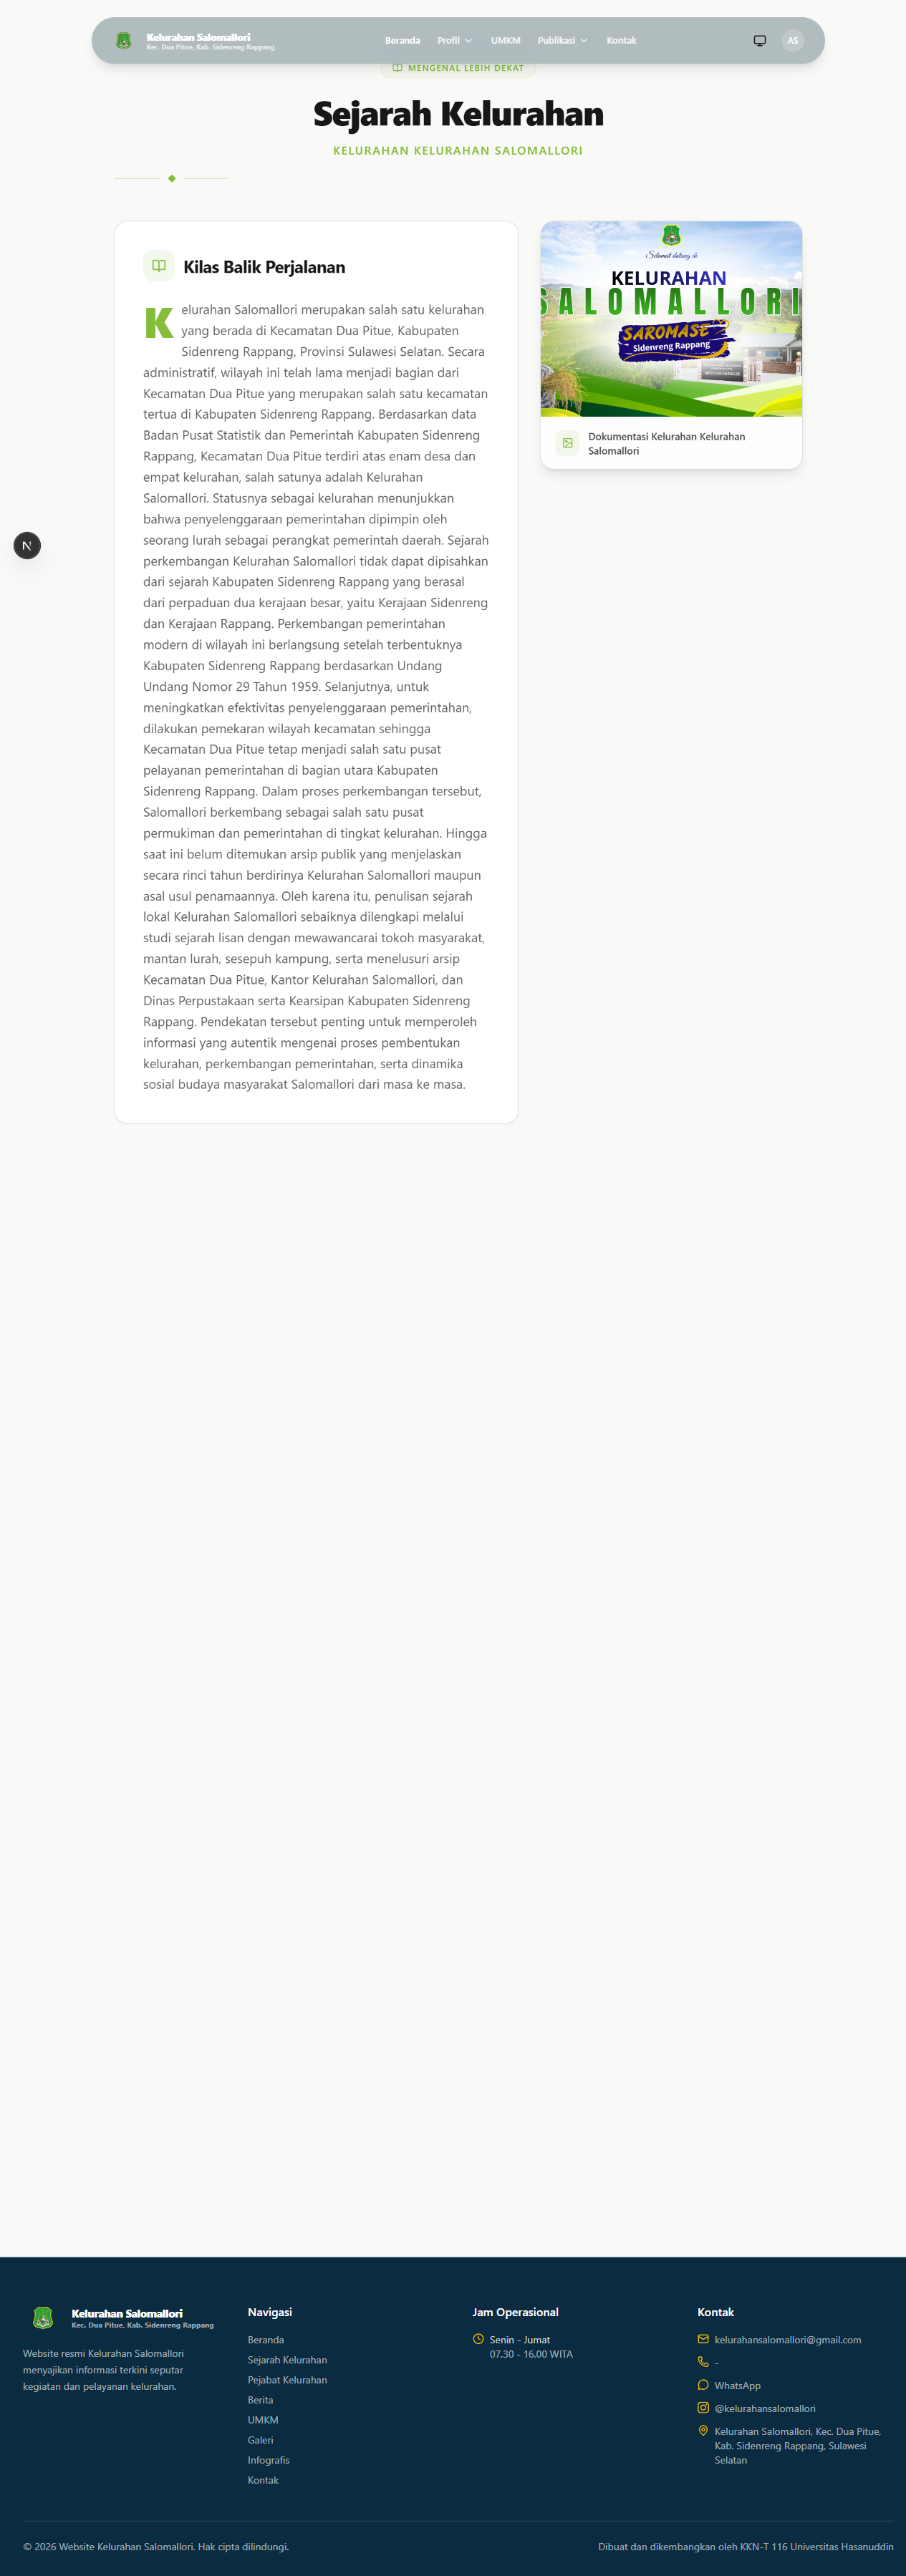
\includegraphics[width=\textwidth]{images/sejarah-kelurahan.png}
        \caption{Halaman Sejarah Kelurahan}
    \end{subfigure}
    \hfill
    \begin{subfigure}{0.45\textwidth}
        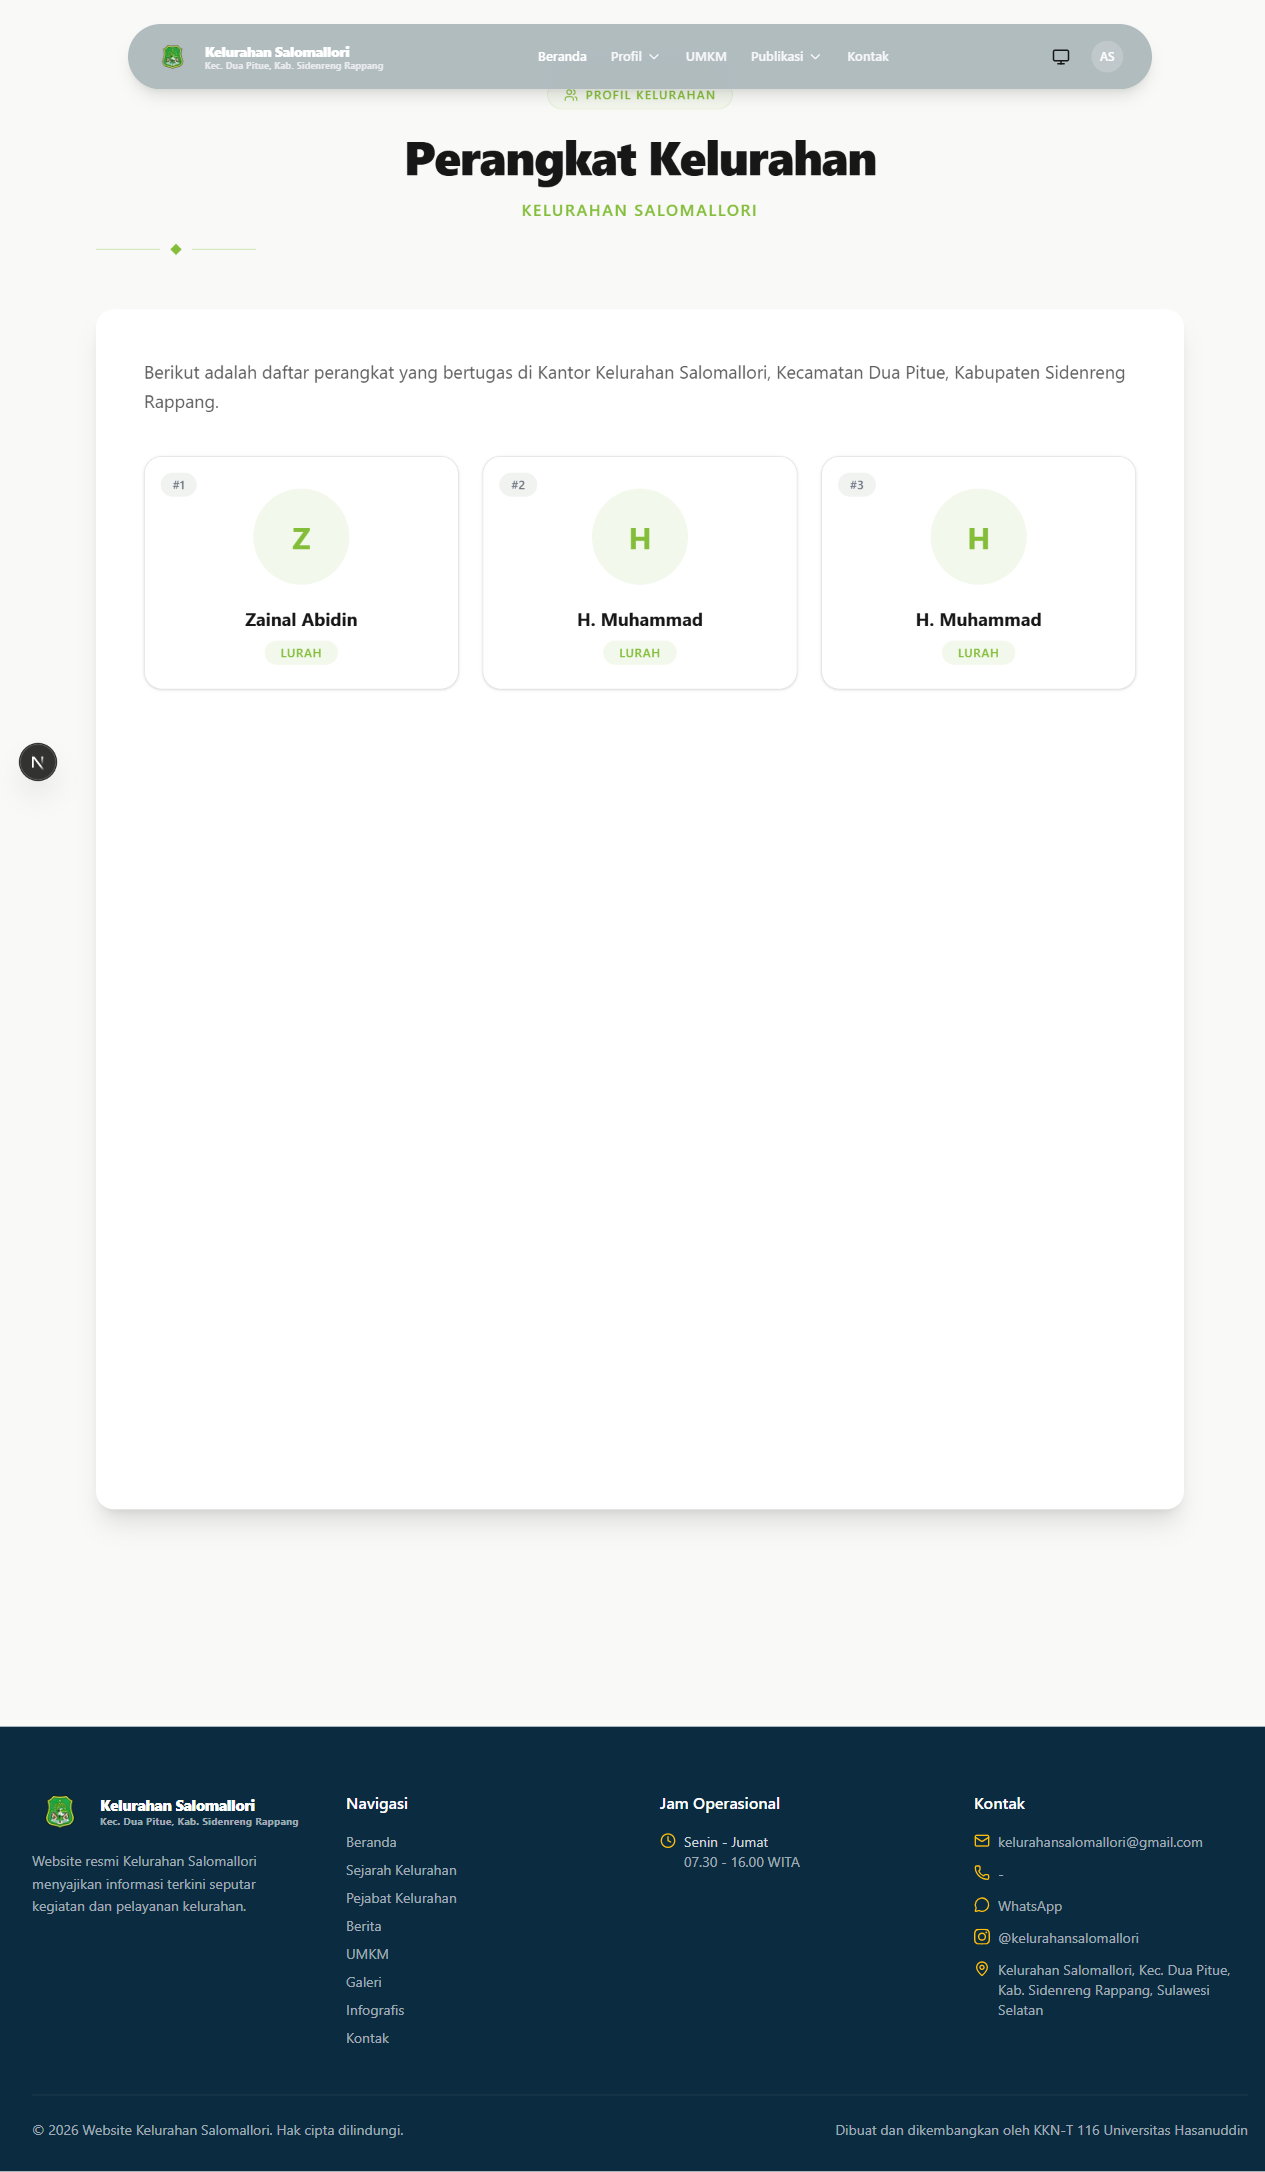
\includegraphics[width=\textwidth]{images/pejabat-kelurahan.png}
        \caption{Halaman Pejabat Kelurahan}
    \end{subfigure}
    \caption{Sub-Menu Profil Kelurahan}
    \label{fig:profil}
\end{figure}

\begin{figure}[H]
    \centering
    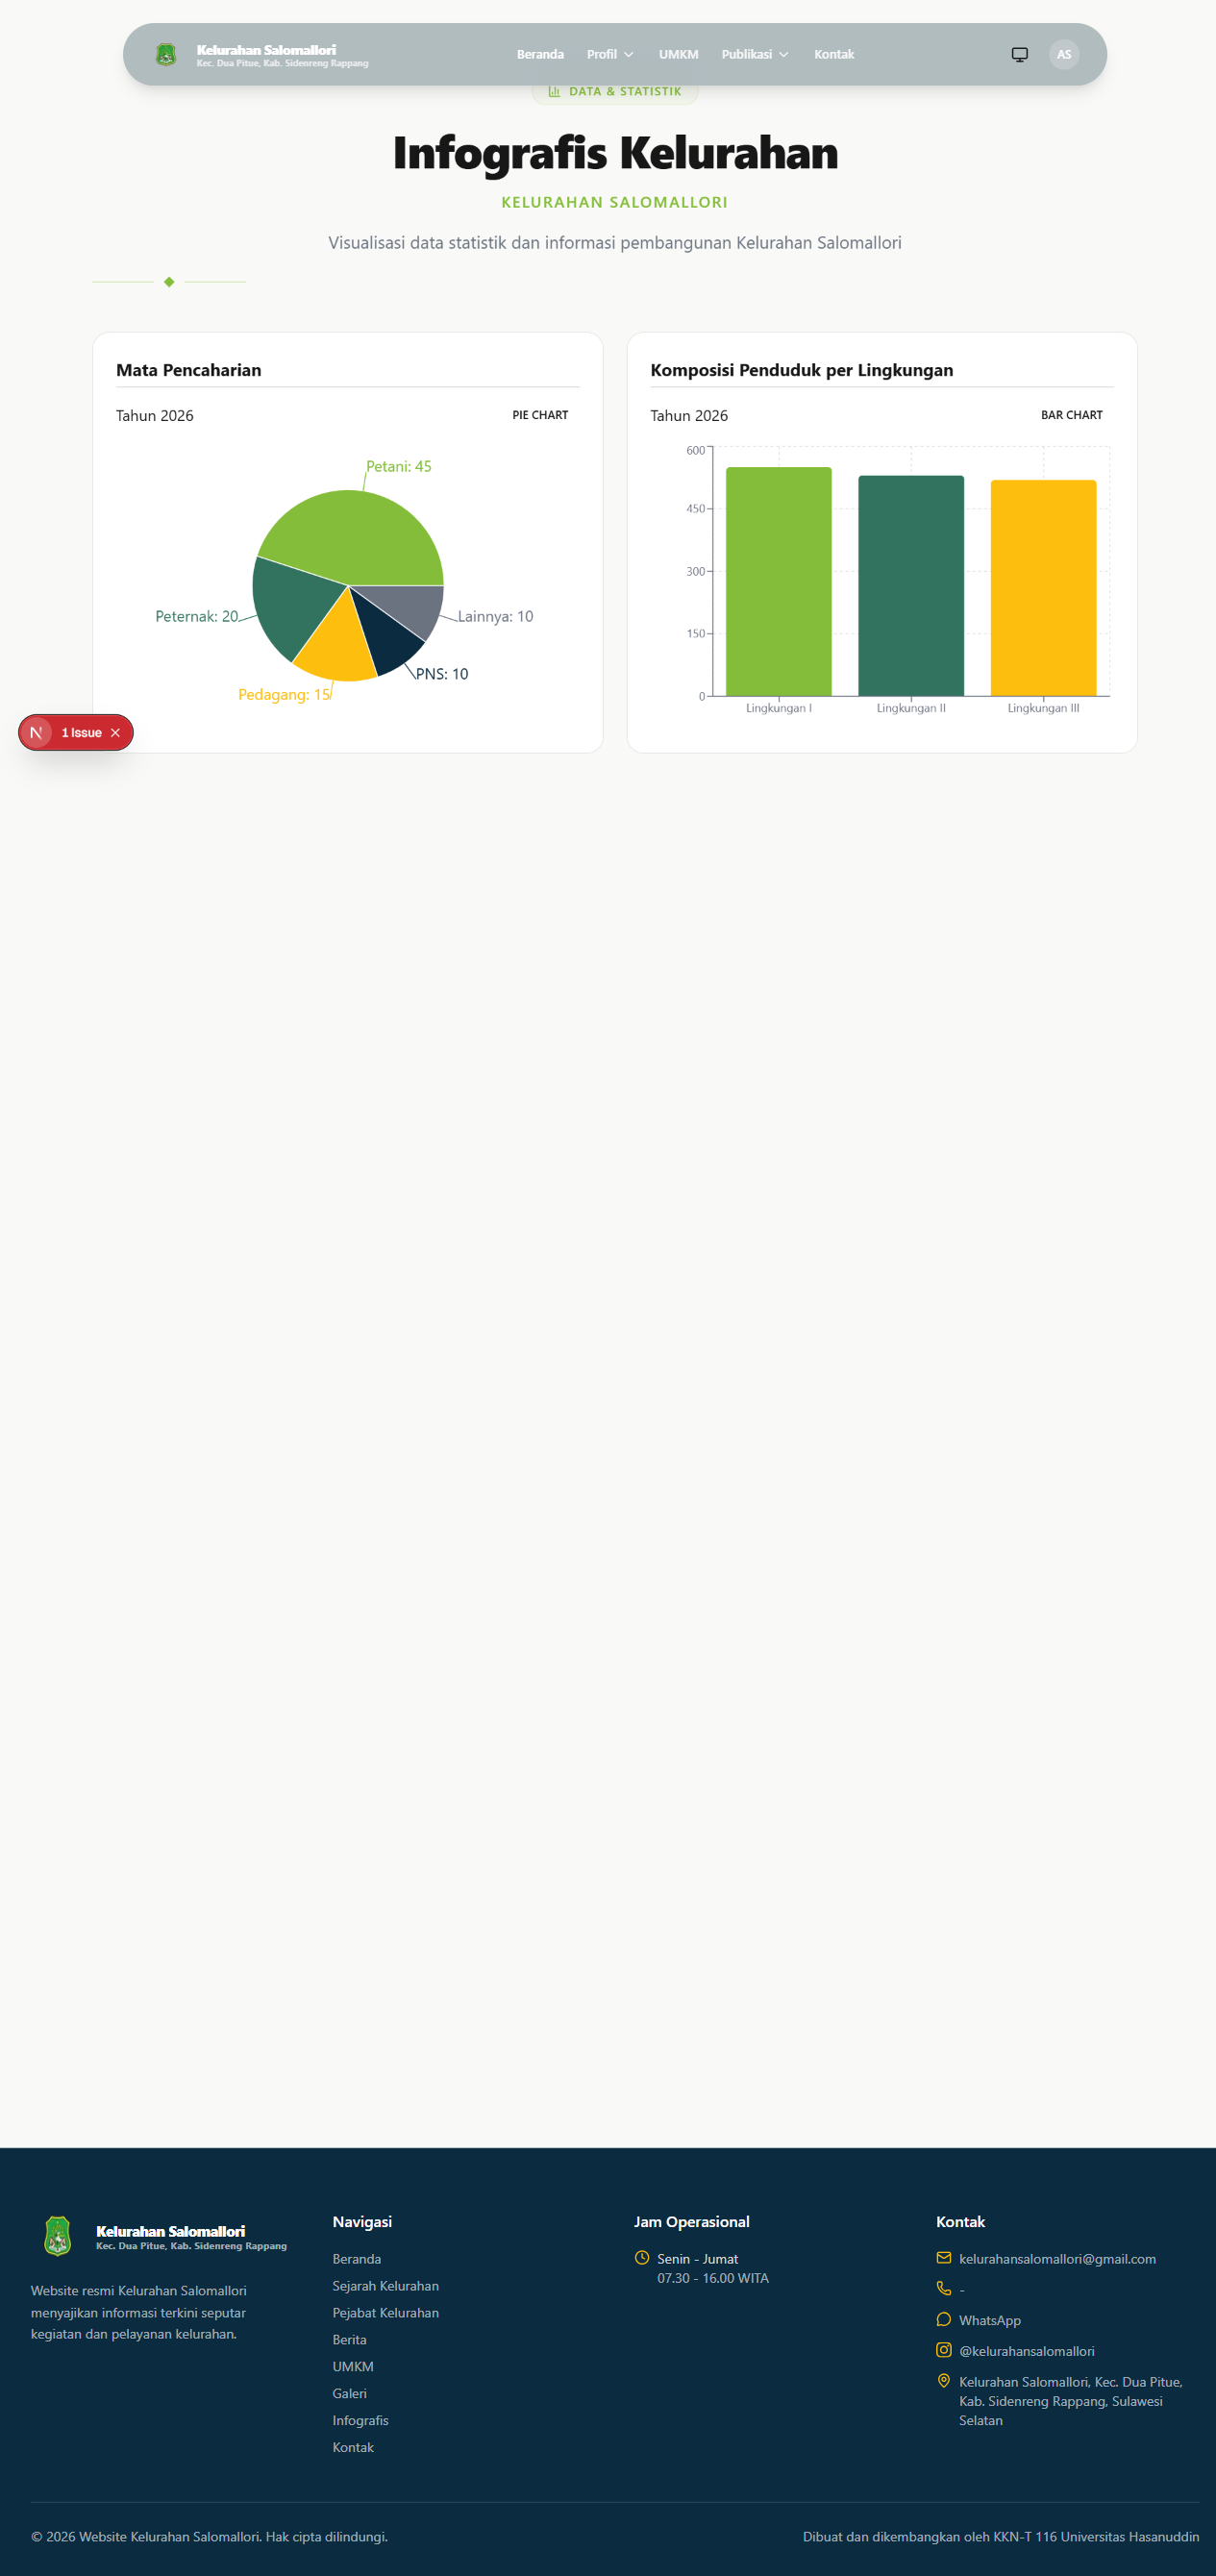
\includegraphics[width=0.85\textwidth]{images/infografis.png}
    \caption{Halaman Infografis -- Visualisasi Data Statistik Kelurahan}
    \label{fig:infografis-pub}
\end{figure}

\subsection{Mengakses Menu Publikasi (Kabar Desa \& Potret Desa)}

Langkah-langkah mengakses menu Publikasi:
\begin{enumerate}[leftmargin=2em, itemsep=2pt]
    \item Arahkan kursor ke menu \textbf{Publikasi} pada navigasi utama;
    \item Muncul \emph{dropdown} yang berisi sub-menu \textbf{Berita} (Kabar Desa) dan \textbf{Galeri Foto} (Potret Desa);
    \item Pilih \textbf{Berita} untuk membaca artikel-artikel terbaru seputar kegiatan kelurahan;
    \item Pilih \textbf{Galeri Foto} untuk melihat dokumentasi foto kegiatan dan keindahan kelurahan.
\end{enumerate}

\begin{figure}[H]
    \centering
    \begin{subfigure}{0.45\textwidth}
        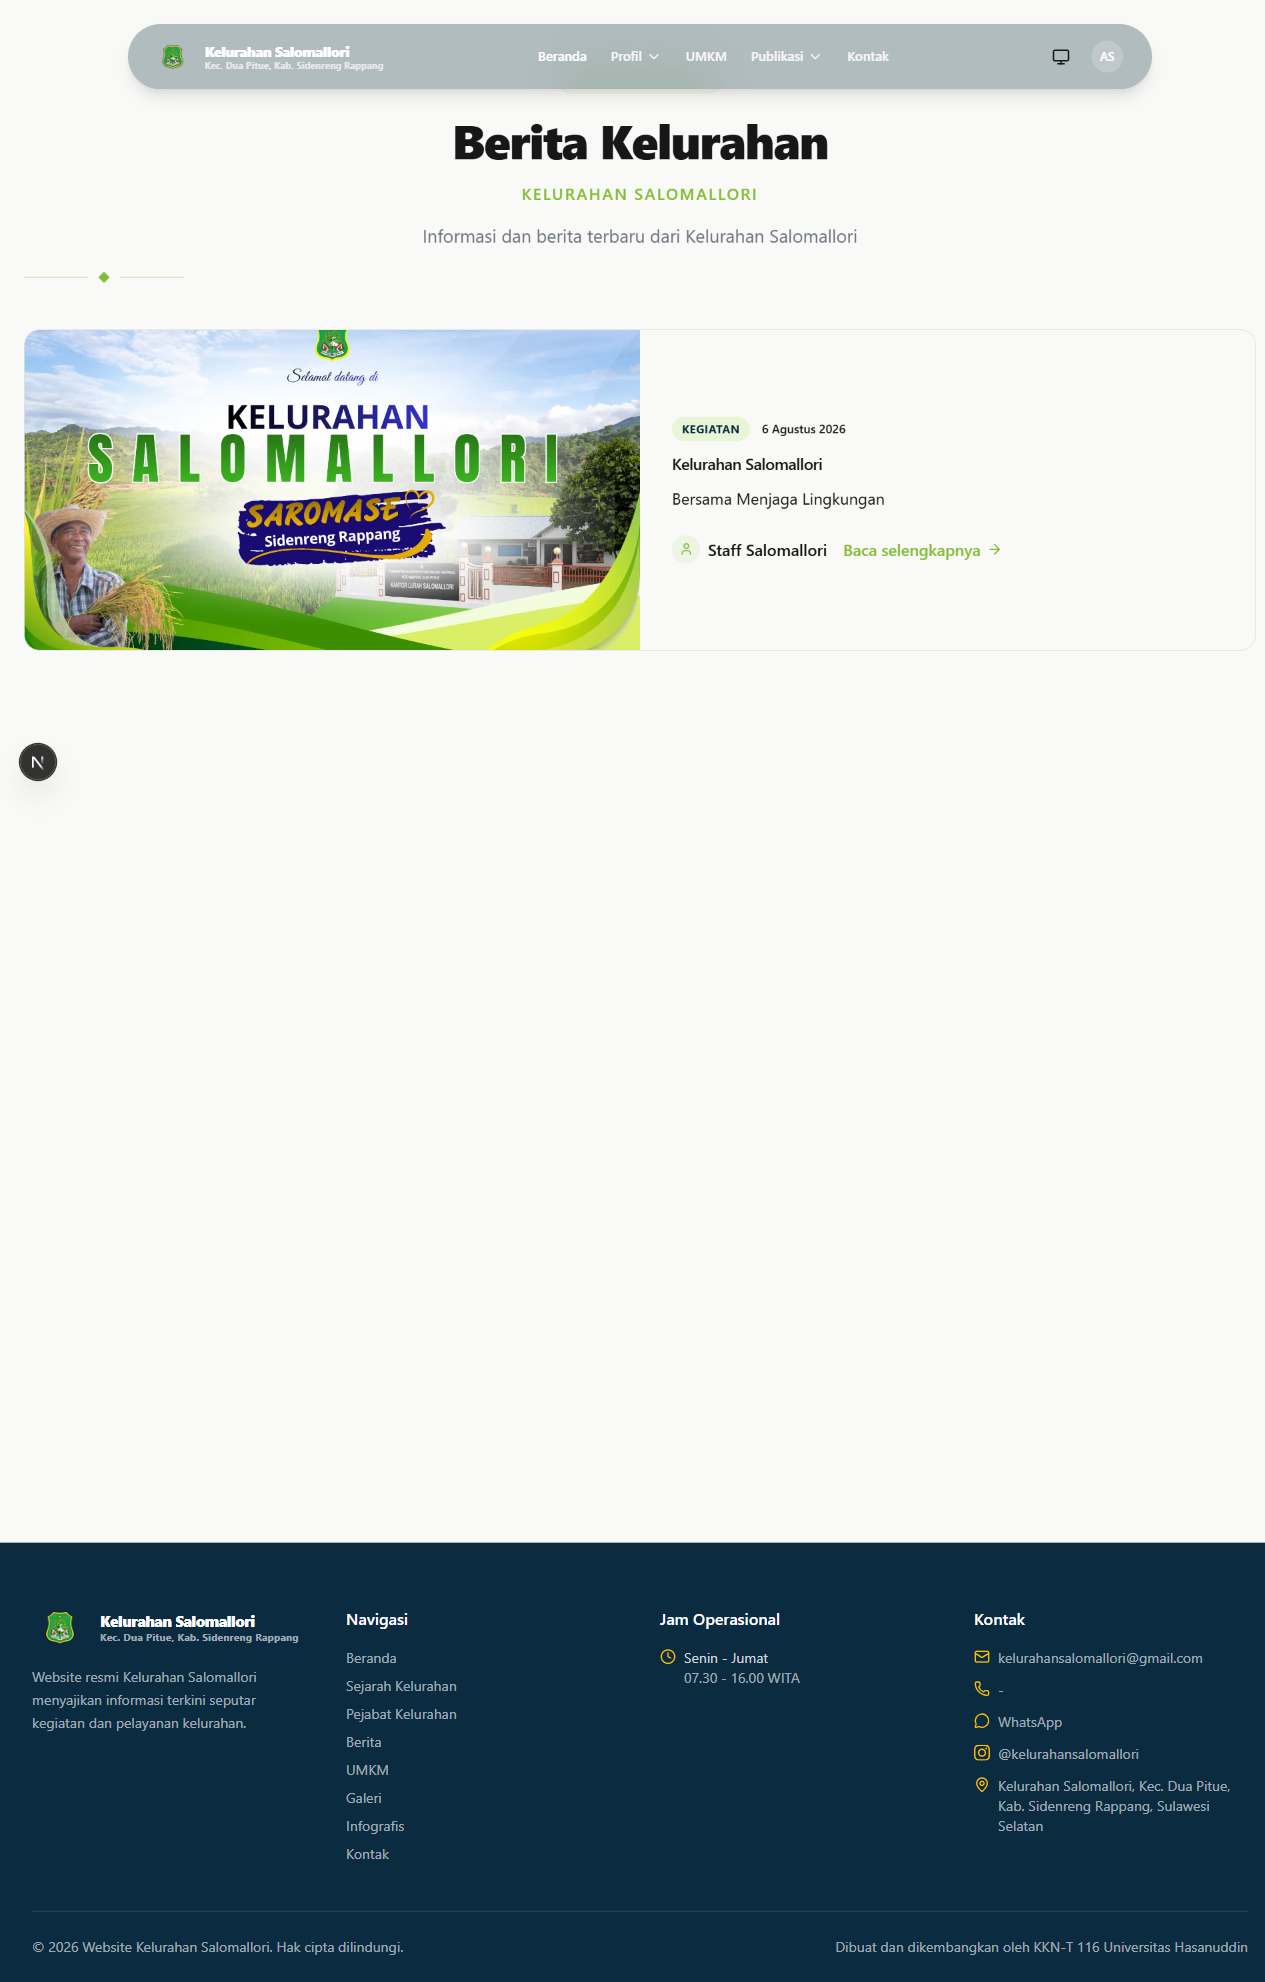
\includegraphics[width=\textwidth]{images/berita.png}
        \caption{Halaman Berita (Kabar Desa)}
    \end{subfigure}
    \hfill
    \begin{subfigure}{0.45\textwidth}
        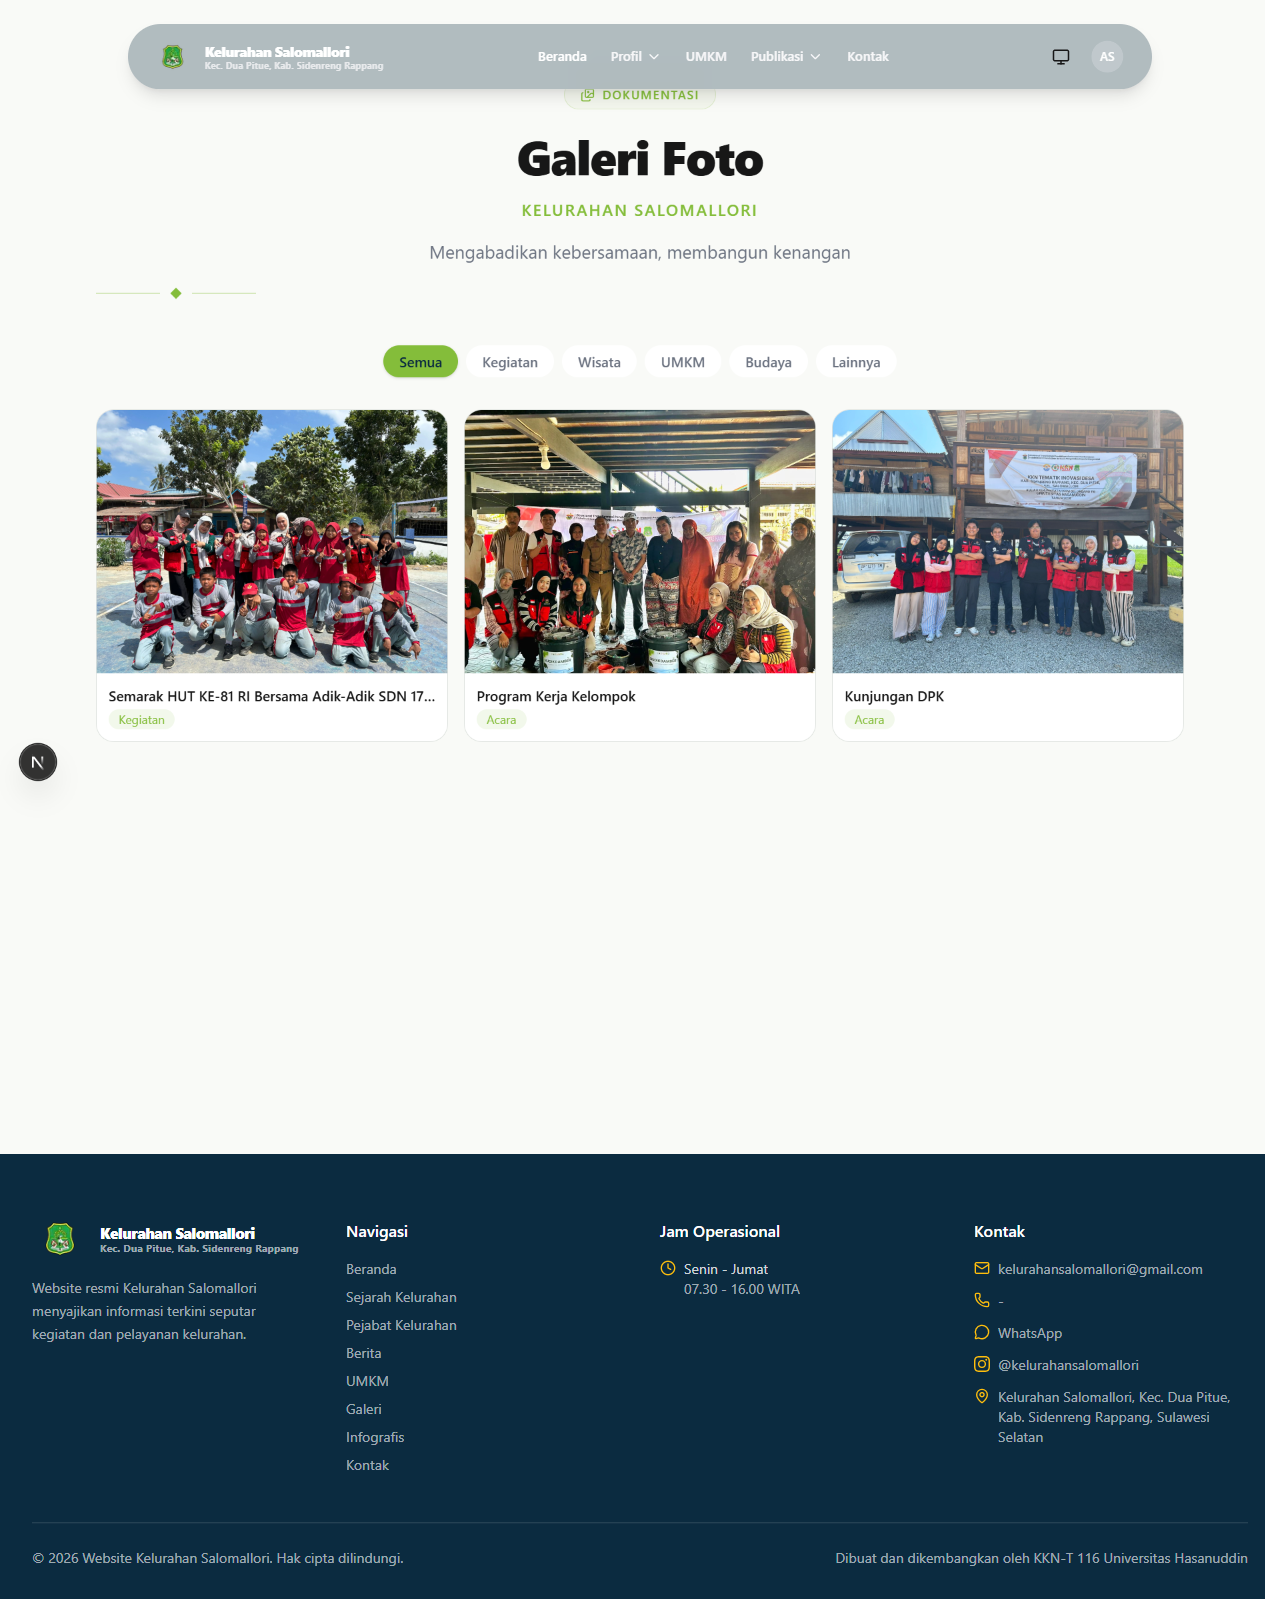
\includegraphics[width=\textwidth]{images/galeri.png}
        \caption{Halaman Galeri Foto (Potret Desa)}
    \end{subfigure}
    \caption{Sub-Menu Publikasi}
    \label{fig:publikasi}
\end{figure}

\subsection{Menjelajahi Katalog Potensi UMKM}

Langkah-langkah menjelajahi katalog UMKM:
\begin{enumerate}[leftmargin=2em, itemsep=2pt]
    \item Pilih menu \textbf{UMKM} pada navigasi utama;
    \item Halaman Katalog UMKM akan menampilkan produk-produk lokal dalam bentuk kartu (\emph{card});
    \item Gunakan kolom \textbf{pencarian} atau \textbf{filter kategori} untuk mencari produk tertentu;
    \item Klik salah satu produk untuk melihat detail lengkap yang mencakup deskripsi, harga, dan informasi kontak penjual;
    \item Hubungi penjual melalui kontak yang tertera pada halaman detail produk.
\end{enumerate}

\begin{figure}[H]
    \centering
    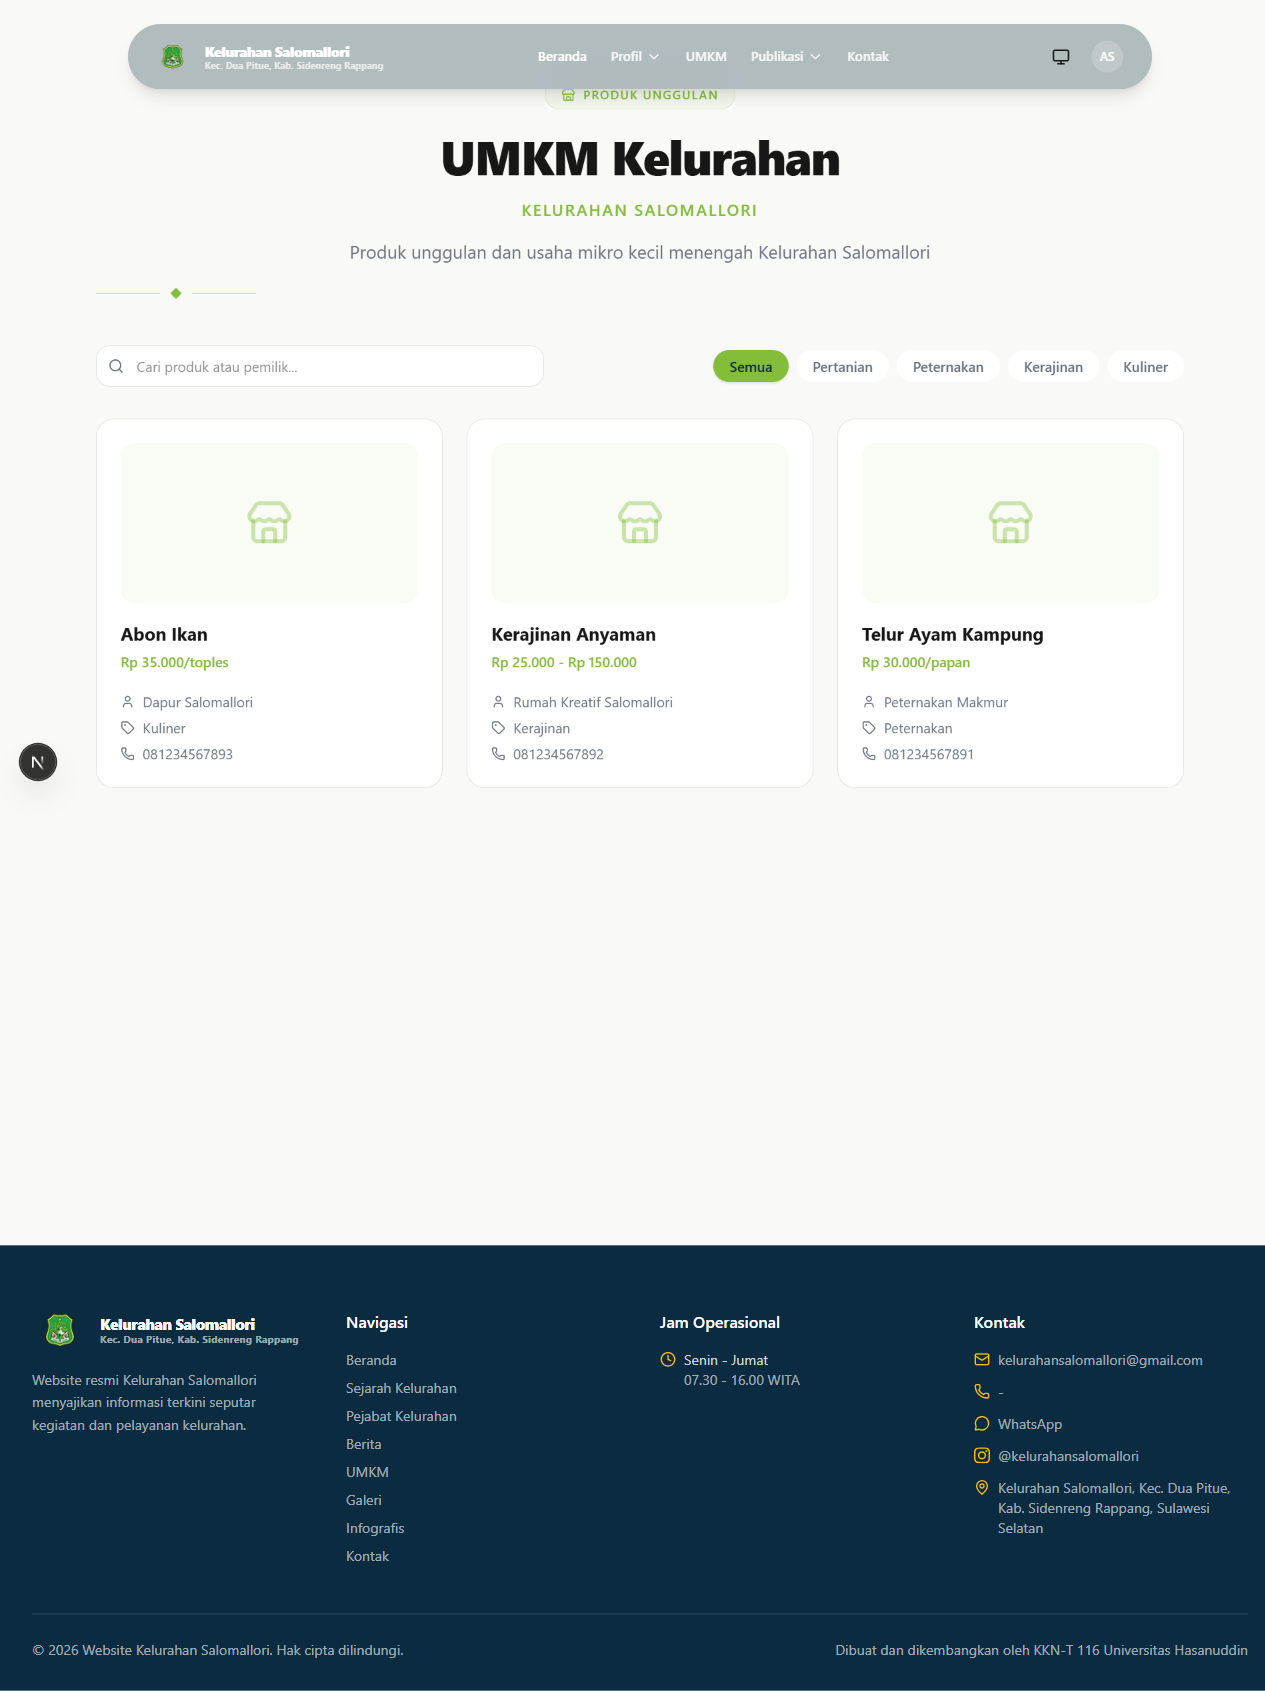
\includegraphics[width=0.85\textwidth]{images/umkm.png}
    \caption{Halaman Katalog UMKM Lokal}
    \label{fig:umkm-pub}
\end{figure}

\subsection{Mengakses Halaman Kontak \& Lokasi}

Informasi kontak dan lokasi kelurahan dapat diakses melalui menu \textbf{Kontak}. Halaman ini menampilkan:
\begin{enumerate}[leftmargin=2em, itemsep=2pt]
    \item Peta lokasi kelurahan melalui \emph{Google Maps embed};
    \item Nomor WhatsApp layanan;
    \item Alamat kantor kelurahan;
    \item Jam operasional layanan.
\end{enumerate}

\begin{figure}[H]
    \centering
    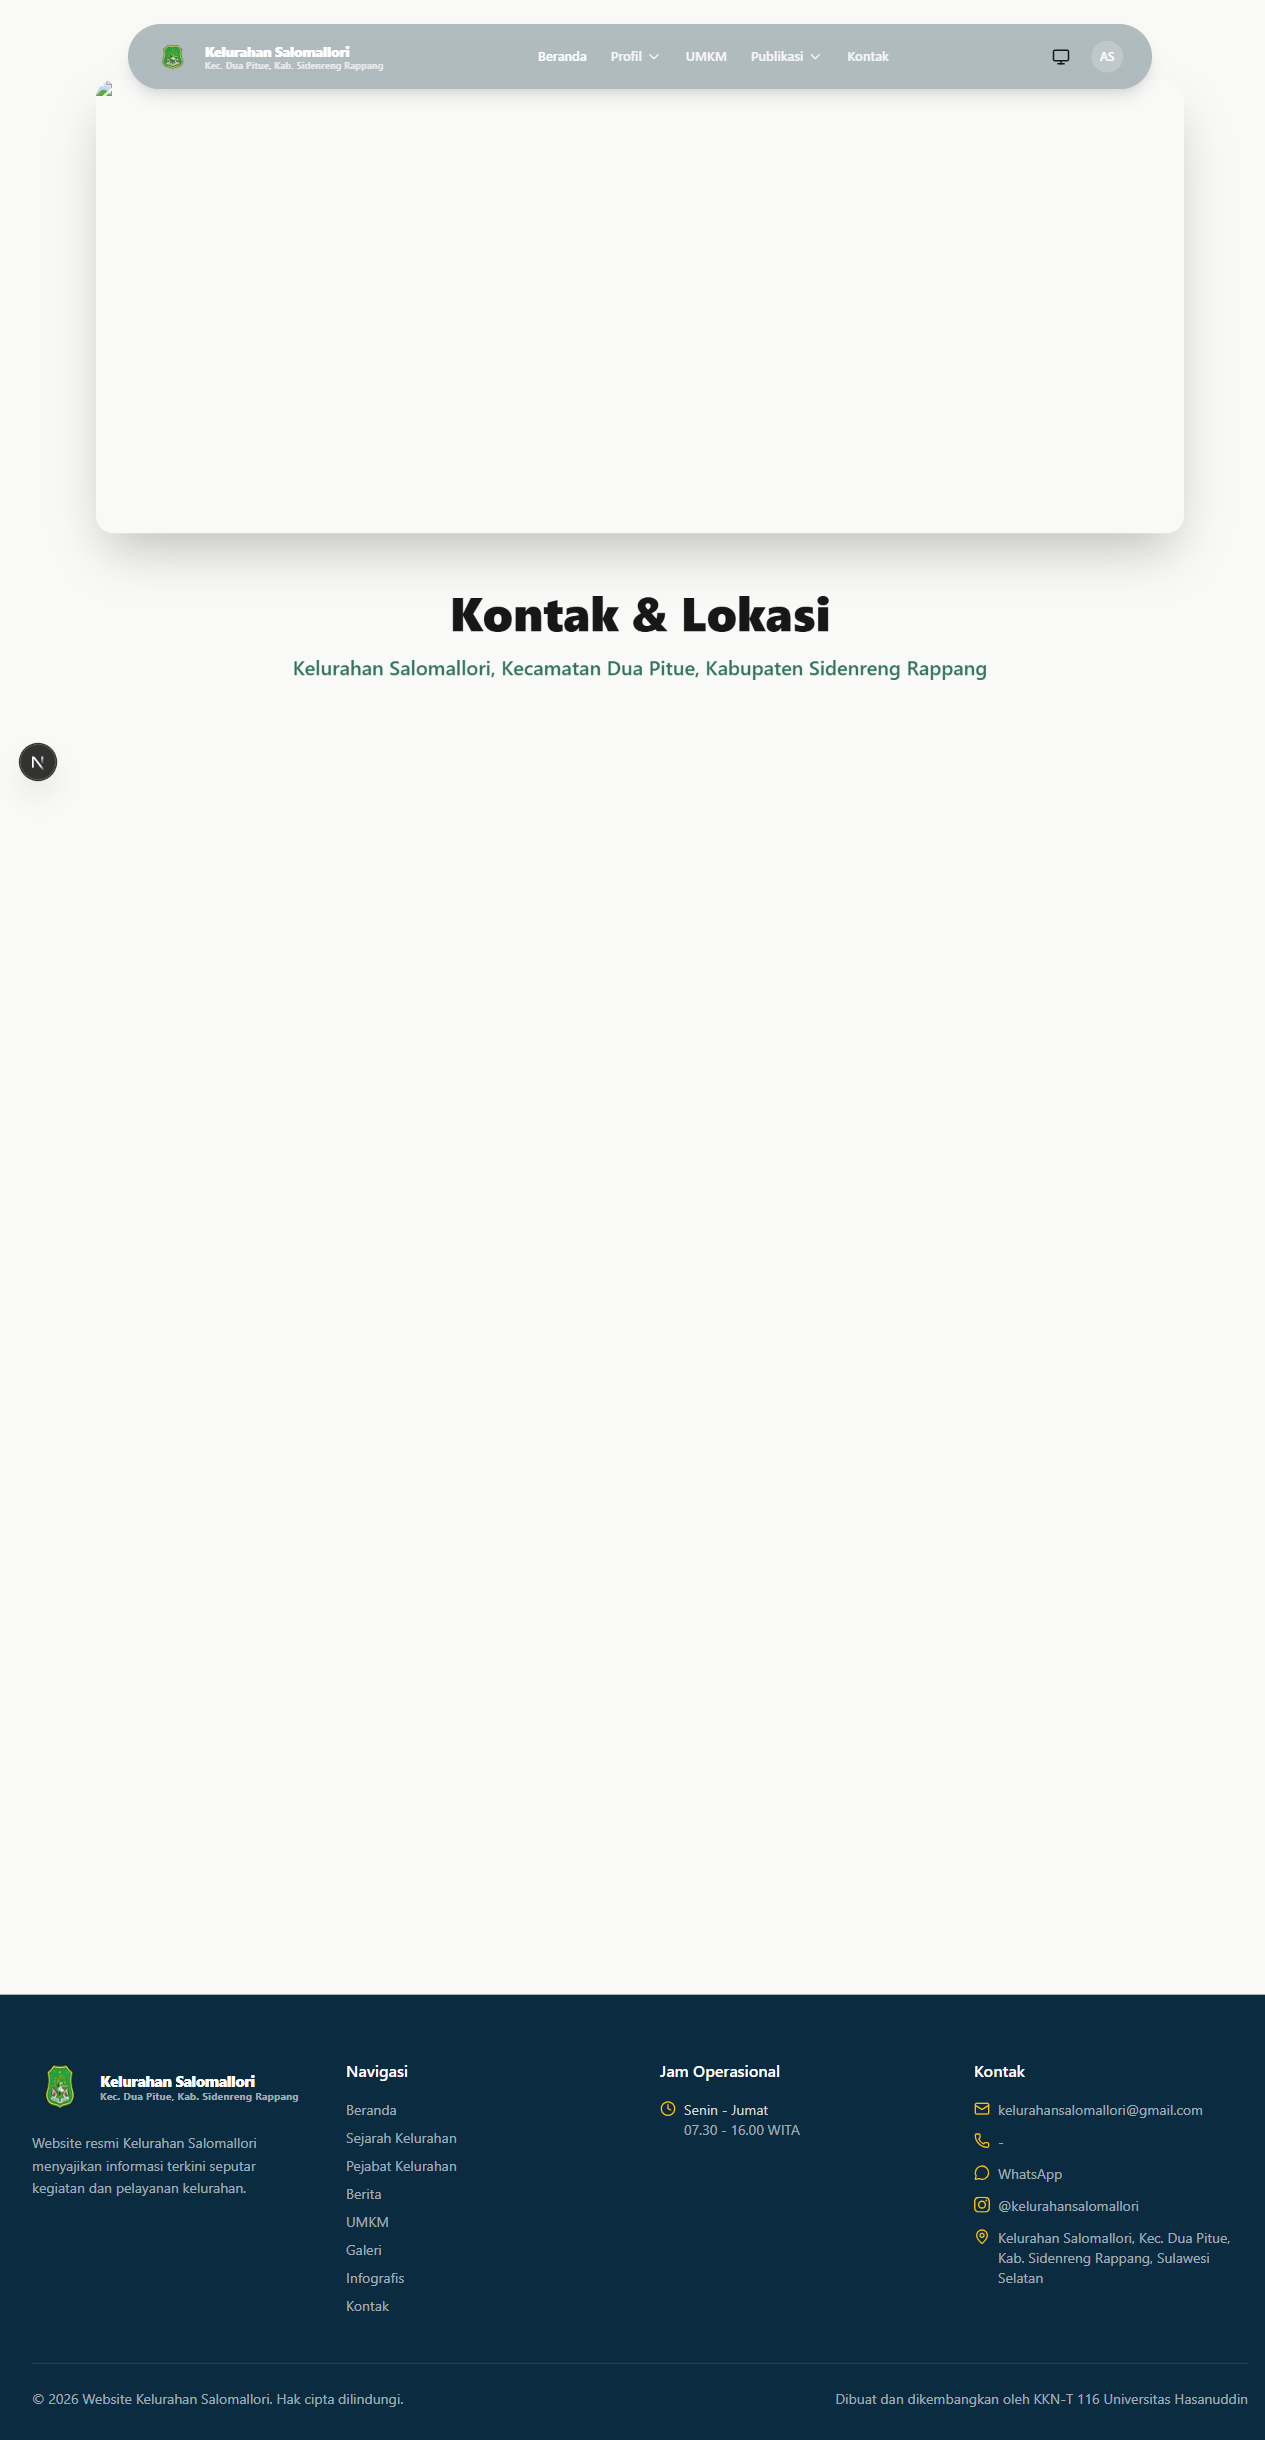
\includegraphics[width=0.85\textwidth]{images/kontak.png}
    \caption{Halaman Kontak \& Lokasi Kelurahan}
    \label{fig:kontak-pub}
\end{figure}

\section{Panduan Administrator \& Editor (Perangkat Kelurahan)}

\subsection{Login ke Dashboard Administrator}

Langkah-langkah masuk ke dashboard:
\begin{enumerate}[leftmargin=2em, itemsep=2pt]
    \item Buka halaman \texttt{/auth/signin} pada browser (atau klik menu \textbf{Masuk} pada navigasi);
    \item Masukkan alamat \textbf{email} dan \textbf{kata sandi} akun yang telah terdaftar;
    \item Klik tombol \textbf{Masuk};
    \item Sistem akan mengarahkan pengguna ke halaman \textbf{Dashboard Overview}.
\end{enumerate}

\begin{figure}[H]
    \centering
    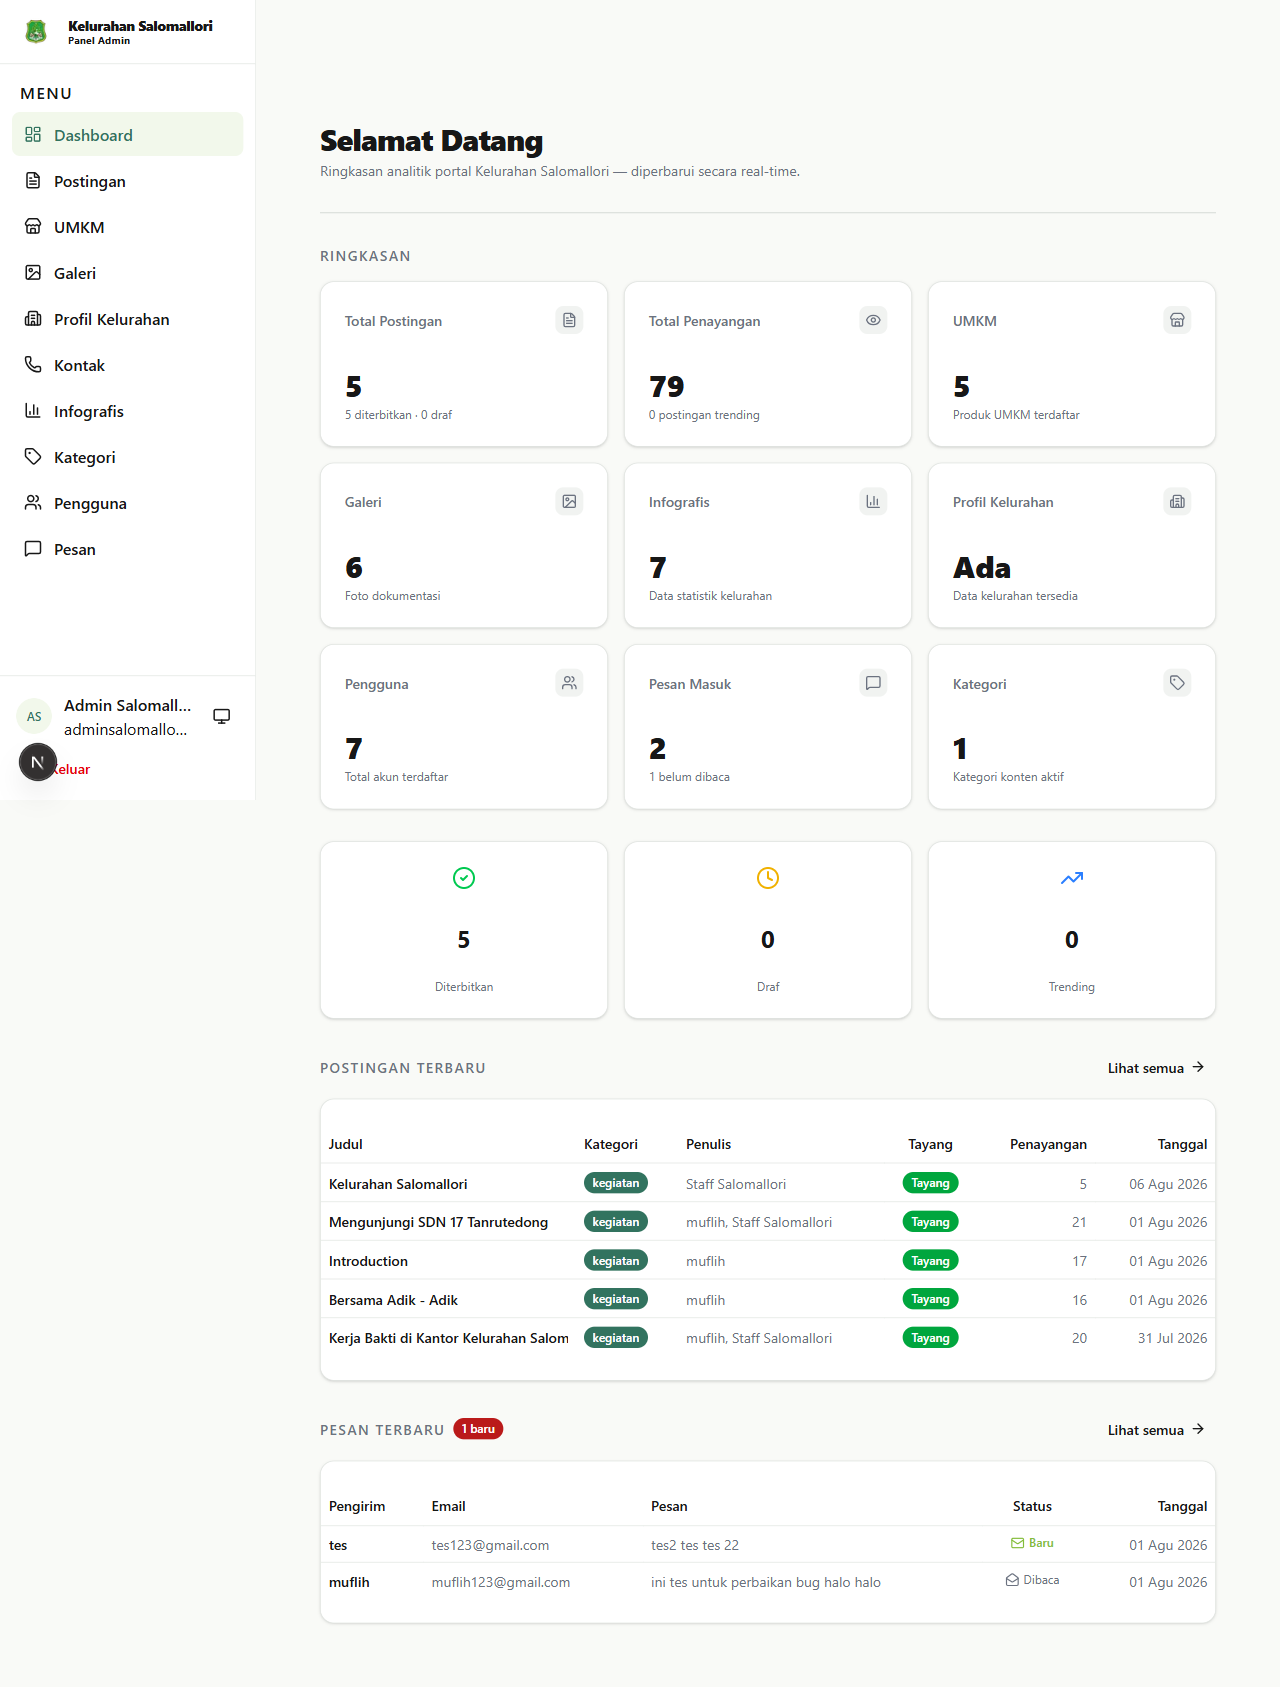
\includegraphics[width=0.85\textwidth]{images/dashboard.png}
    \caption{Dashboard Overview Administrator}
    \label{fig:dashboard-admin}
\end{figure}

Halaman Dashboard Overview menampilkan ringkasan analitik portal yang diperbarui secara real-time, antara lain total postingan, total penayangan, jumlah UMKM, jumlah foto galeri, jumlah infografis, ketersediaan profil kelurahan, jumlah pengguna, dan jumlah pesan masuk.

\subsection{Mengelola Informasi Profil Kelurahan \& Perangkat}

Menu \textbf{Profil Kelurahan} pada dashboard digunakan untuk memperbarui data identitas kelurahan. Langkah-langkahnya:
\begin{enumerate}[leftmargin=2em, itemsep=2pt]
    \item Pilih menu \textbf{Profil Kelurahan} pada sidebar dashboard;
    \item Perbarui data identitas kelurahan, antara lain:
    \begin{itemize}[leftmargin=2em, itemsep=2pt]
        \item Luas wilayah (saat ini \textbf{7,63 km²});
        \item Jumlah penduduk (saat ini \textbf{3.234 jiwa});
        \item Jumlah kepala keluarga (saat ini \textbf{1.077 KK});
        \item Jumlah lingkungan (saat ini \textbf{3 lingkungan});
        \item Sejarah kelurahan;
        \item Batas wilayah (Utara, Timur, Selatan, Barat);
        \item Visi dan misi kelurahan;
        \item Foto Kepala Desa.
    \end{itemize}
    \item Kelola daftar \textbf{Pejabat/Perangkat Kelurahan} dengan mengatur urutan tampilan (\emph{urutan}) dan foto masing-masing perangkat;
    \item Klik \textbf{Simpan} untuk menyimpan perubahan.
\end{enumerate}

\begin{figure}[H]
    \centering
    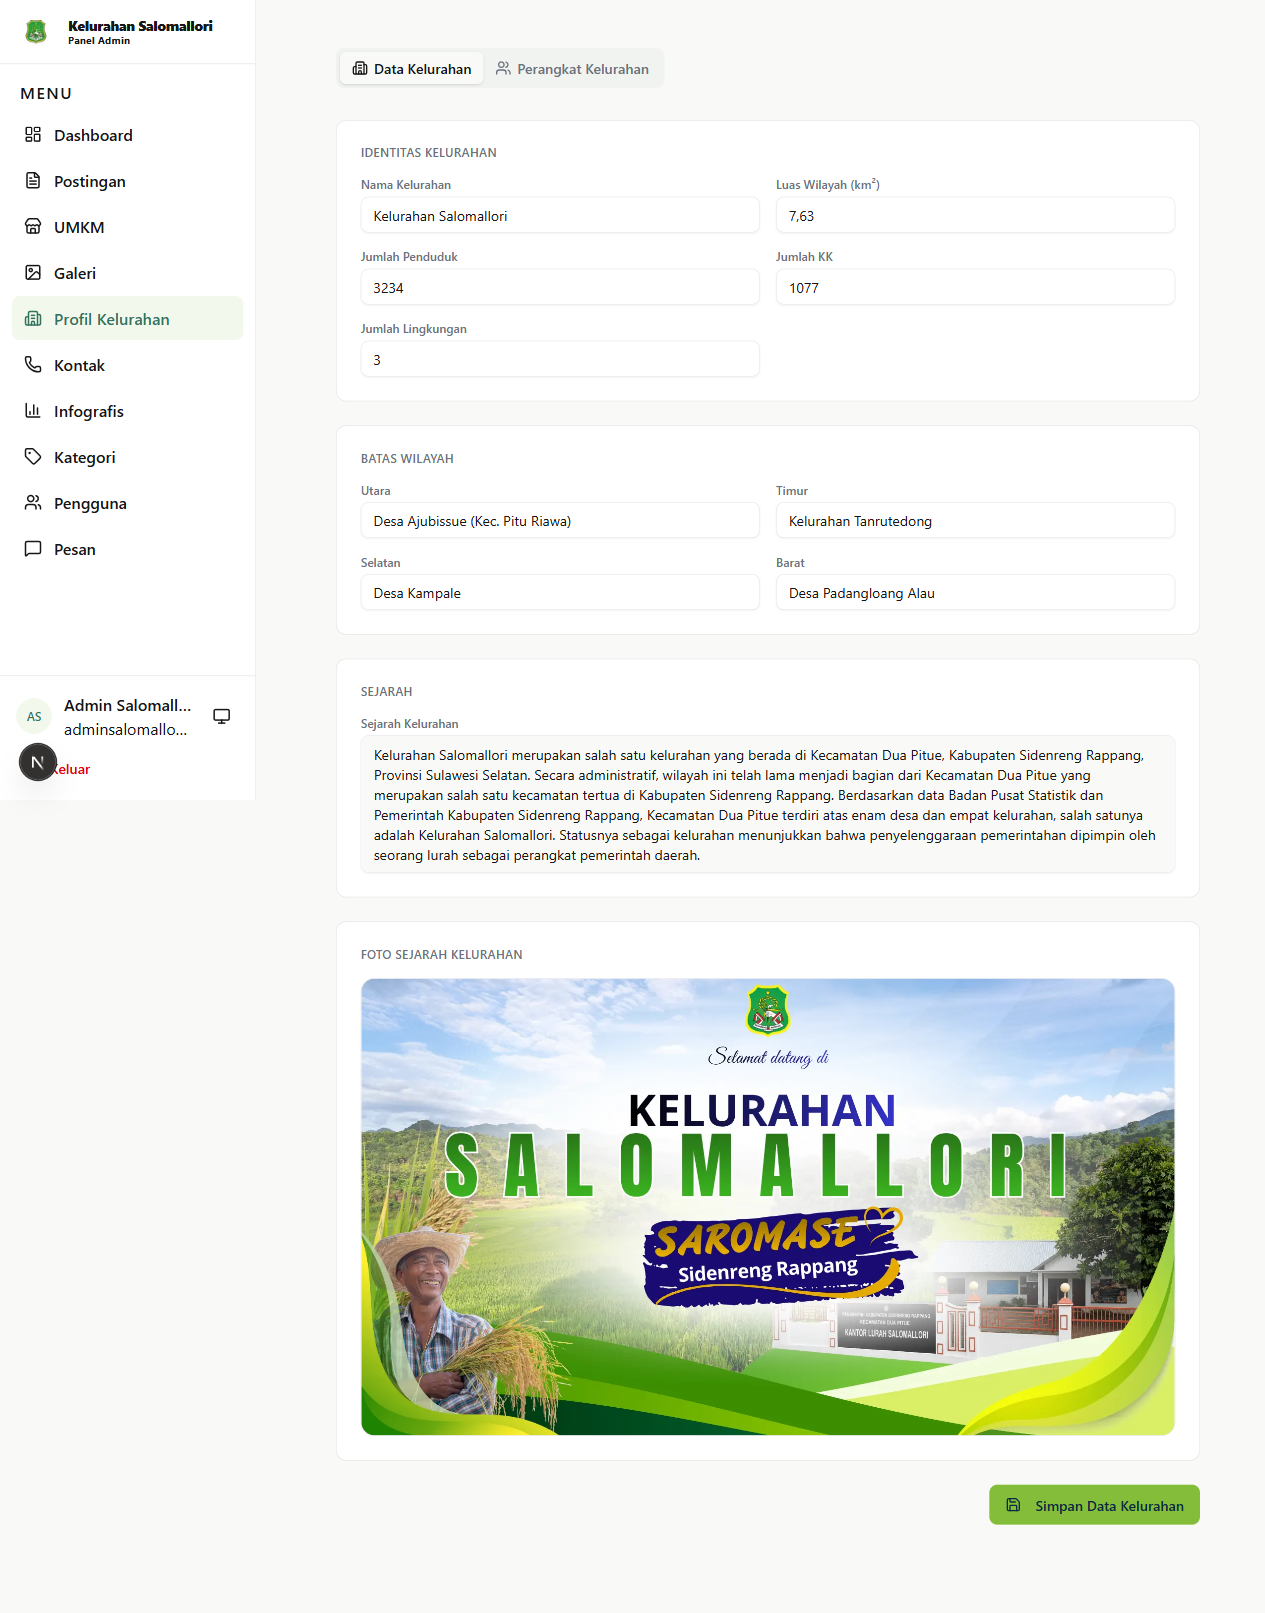
\includegraphics[width=0.85\textwidth]{images/admin-profil-desa.png}
    \caption{Form Pendataan Profil Kelurahan \& Perangkat}
    \label{fig:admin-profil}
\end{figure}

\subsection{Mengelola Publikasi Berita \& Galeri Foto}

\subsubsection{Mengelola Berita (Kabar Desa)}

Langkah-langkah menambah atau mengedit berita:
\begin{enumerate}[leftmargin=2em, itemsep=2pt]
    \item Pilih menu \textbf{Postingan} pada sidebar dashboard;
    \item Klik tombol \textbf{Buat Postingan} untuk menulis berita baru;
    \item Isi \textbf{Judul}, \textbf{Konten}, \textbf{Kategori}, \textbf{Gambar Sampul}, dan pengaturan lainnya;
    \item Gunakan \textbf{TipTap Rich Text Editor} untuk memformat konten (tebal, miring, heading, daftar, link, dan lain-lain);
    \item Klik \textbf{Terbitkan} untuk mempublikasikan berita ke halaman publik;
    \item Untuk mengedit berita, klik tombol \textbf{Edit} pada daftar postingan.
\end{enumerate}

\begin{figure}[H]
    \centering
    \begin{subfigure}{0.45\textwidth}
        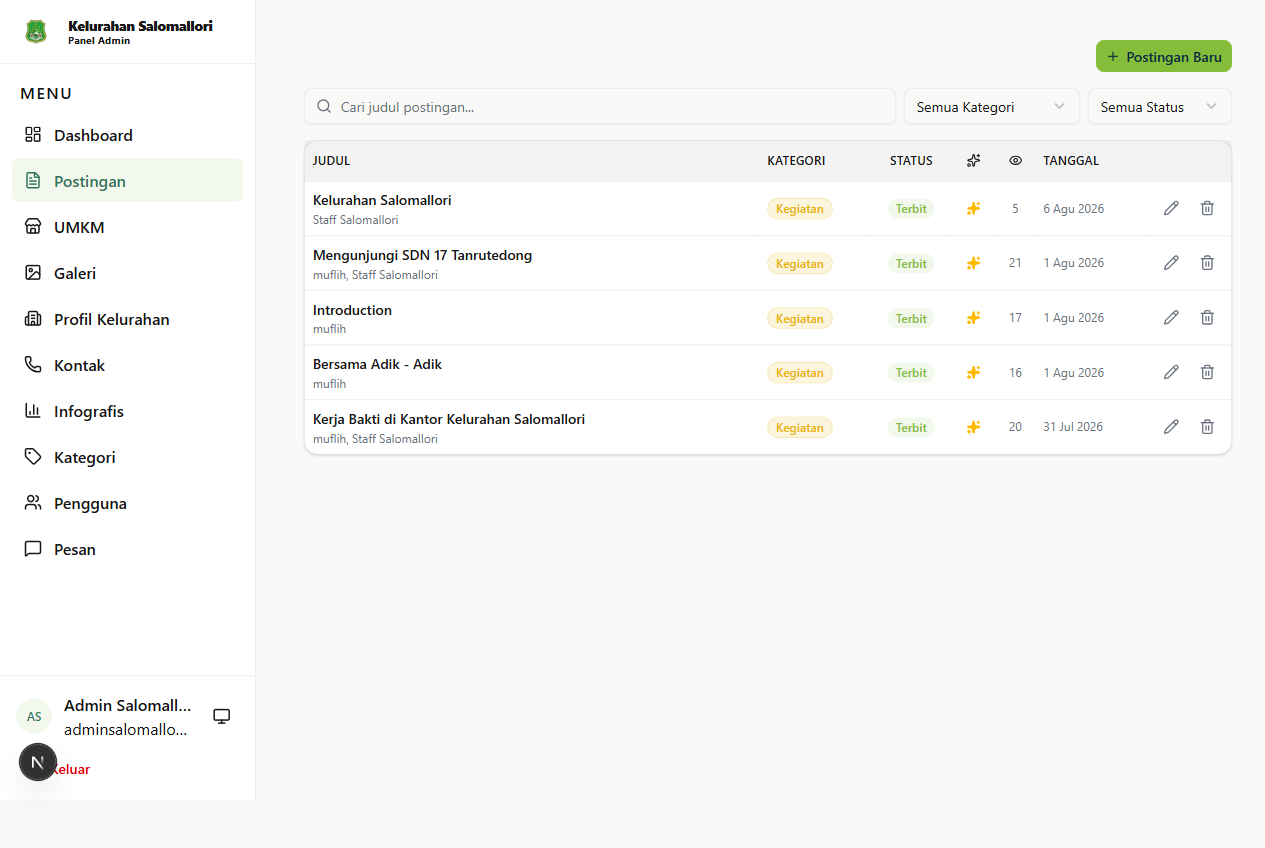
\includegraphics[width=\textwidth]{images/admin-posts.png}
        \caption{Daftar Postingan Berita}
    \end{subfigure}
    \hfill
    \begin{subfigure}{0.45\textwidth}
        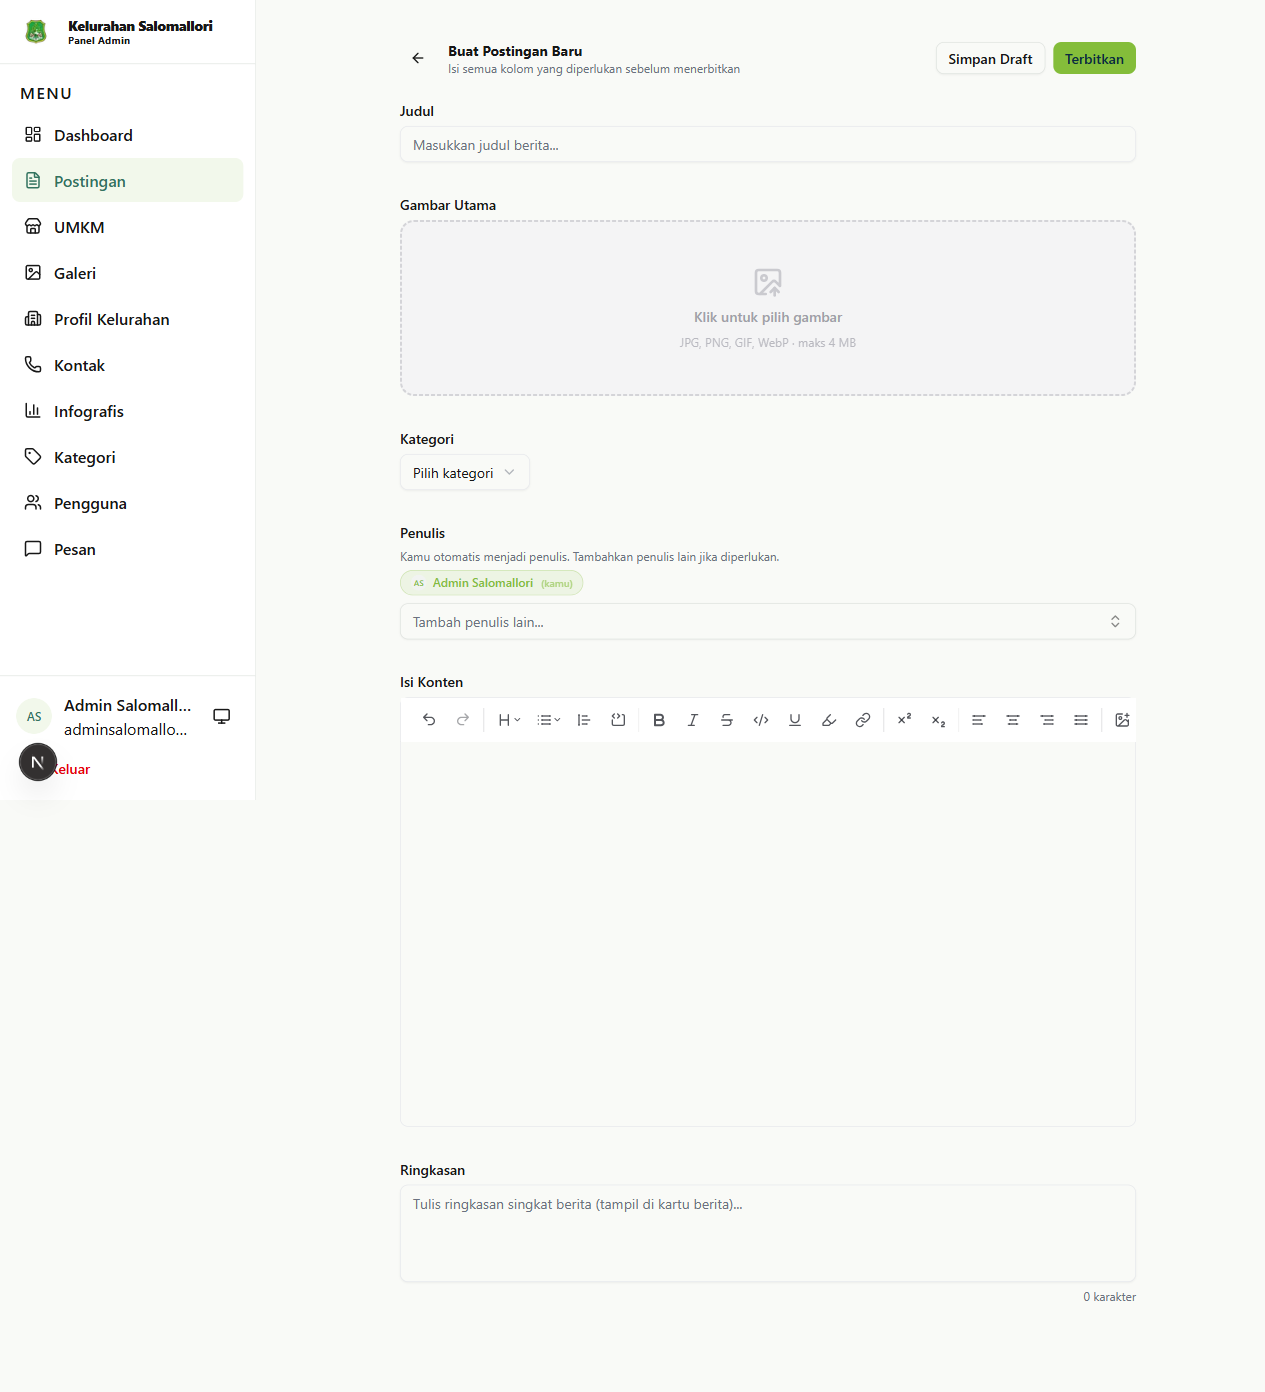
\includegraphics[width=\textwidth]{images/admin-posts-create.png}
        \caption{Form Penulisan Berita dengan TipTap Editor}
    \end{subfigure}
    \caption{Pengelolaan Publikasi Berita}
    \label{fig:admin-posts}
\end{figure}

\subsubsection{Mengelola Galeri Foto (Potret Desa)}

Langkah-langkah mengunggah foto kegiatan:
\begin{enumerate}[leftmargin=2em, itemsep=2pt]
    \item Pilih menu \textbf{Galeri} pada sidebar dashboard;
    \item Klik tombol \textbf{Tambah Foto};
    \item Lengkapi \textbf{Judul} dan \textbf{Kategori} foto;
    \item Unggah gambar melalui fitur \emph{upload} yang terhubung dengan layanan \textbf{Cloudinary};
    \item Klik \textbf{Simpan}; foto akan muncul pada halaman Galeri publik.
\end{enumerate}

\begin{figure}[H]
    \centering
    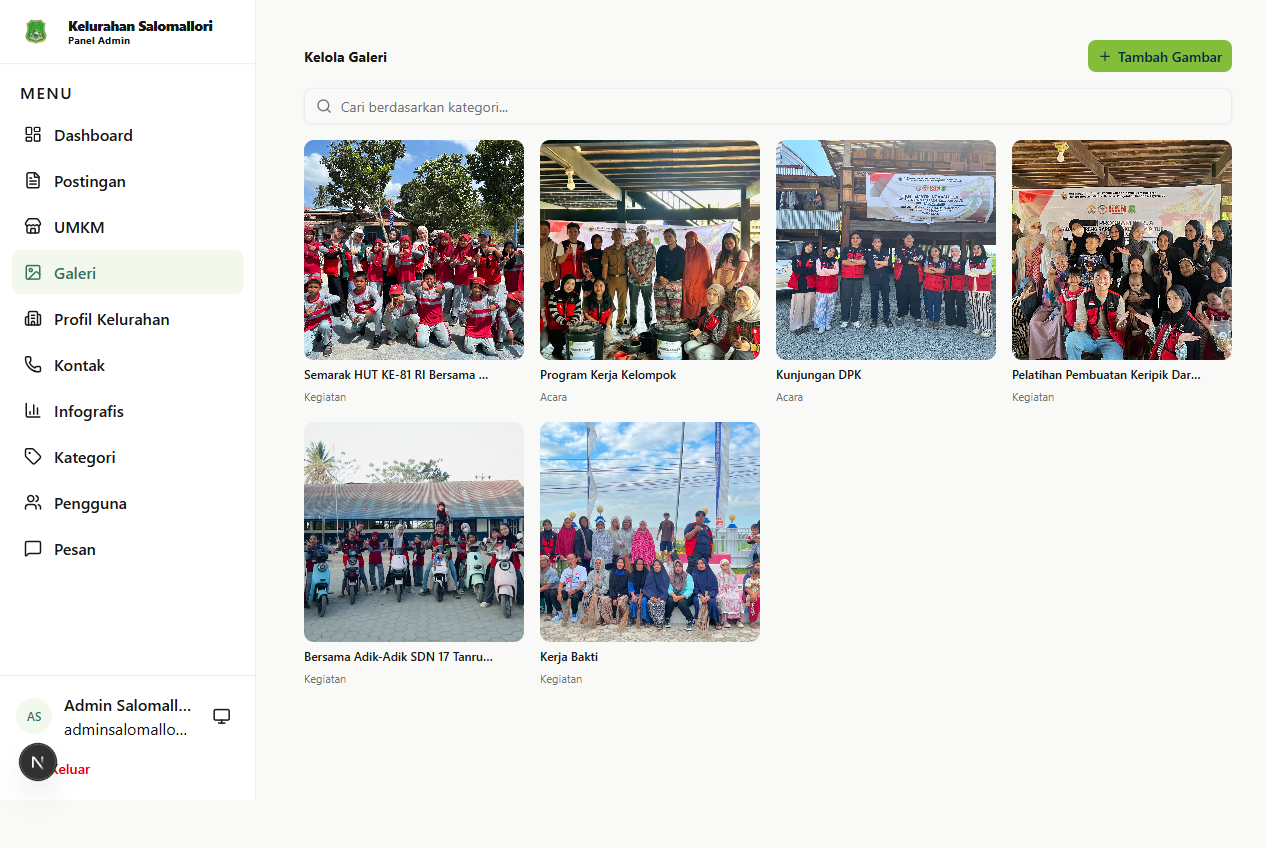
\includegraphics[width=0.85\textwidth]{images/admin-galeri.png}
    \caption{Halaman Kelola Galeri Foto}
    \label{fig:admin-galeri}
\end{figure}

\subsection{Mengelola Katalog UMKM}

Langkah-langkah menambahkan produk UMKM:
\begin{enumerate}[leftmargin=2em, itemsep=2pt]
    \item Pilih menu \textbf{UMKM} pada sidebar dashboard;
    \item Klik tombol \textbf{Tambah UMKM};
    \item Isi \textbf{Nama Produk}, \textbf{Deskripsi}, \textbf{Harga}, \textbf{Kategori}, \textbf{Nama Pemilik}, dan \textbf{Kontak};
    \item Unggah \textbf{Gambar Produk} melalui fitur \emph{upload} Cloudinary;
    \item Klik \textbf{Simpan}; produk akan tampil pada halaman Katalog UMKM publik.
\end{enumerate}

\begin{figure}[H]
    \centering
    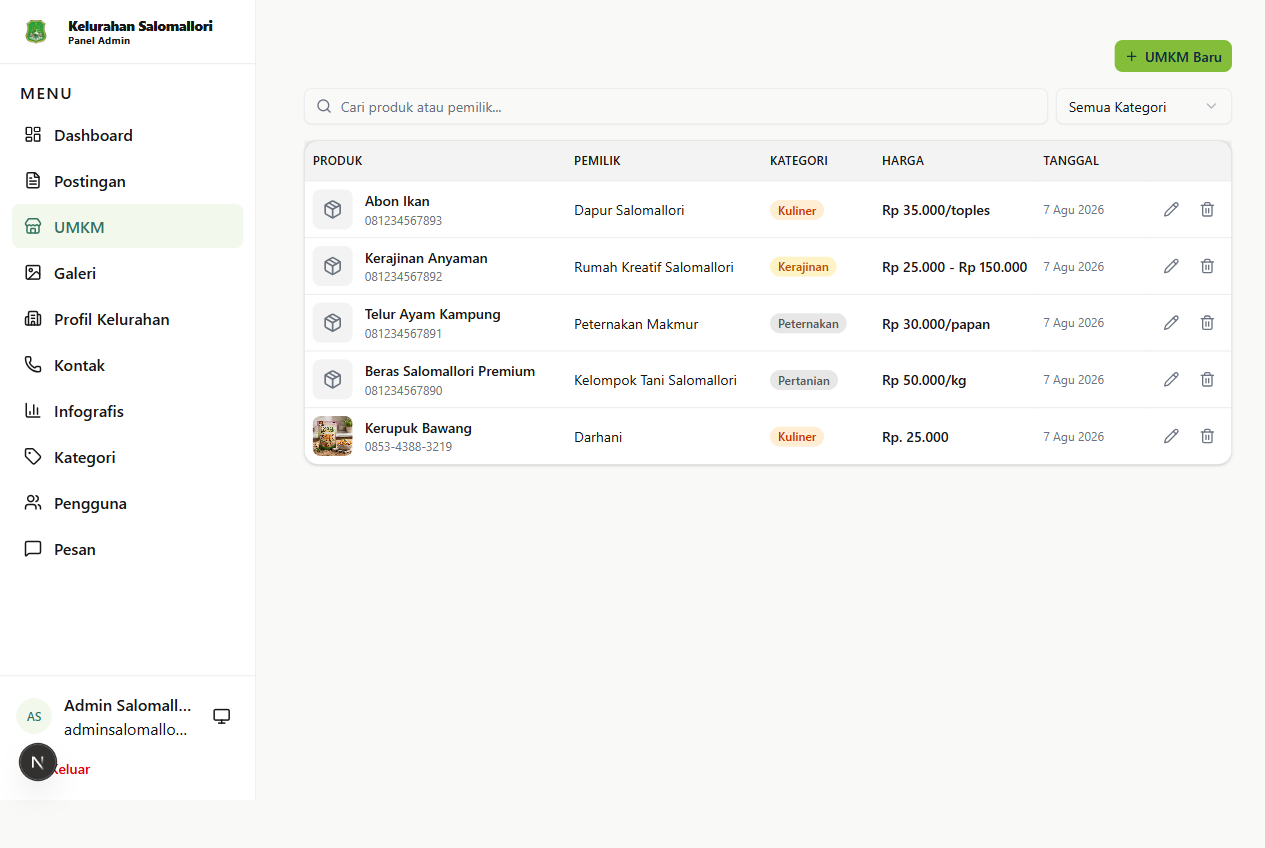
\includegraphics[width=0.85\textwidth]{images/admin-umkm.png}
    \caption{Halaman Kelola Katalog UMKM}
    \label{fig:admin-umkm}
\end{figure}

\subsection{Mengelola Infografis \& Data Statistik}

Langkah-langkah memperbarui infografis:
\begin{enumerate}[leftmargin=2em, itemsep=2pt]
    \item Pilih menu \textbf{Infografis} pada sidebar dashboard;
    \item Pilih data infografis yang akan diperbarui atau klik \textbf{Tambah} untuk membuat infografis baru;
    \item Lengkapi \textbf{Judul} dan \textbf{Tahun} data;
    \item Perbarui \textbf{dataJson} yang berisi data statistik kelurahan;
    \item Pilih \textbf{Tipe Chart} yang diinginkan, antara lain \emph{Bar Chart}, \emph{Line Chart}, \emph{Pie Chart}, \emph{Doughnut Chart}, \emph{Area Chart}, atau \emph{Stat Cards};
    \item Klik \textbf{Simpan}; visualisasi akan tampil pada halaman Infografis di bawah menu Profil.
\end{enumerate}

\begin{figure}[H]
    \centering
    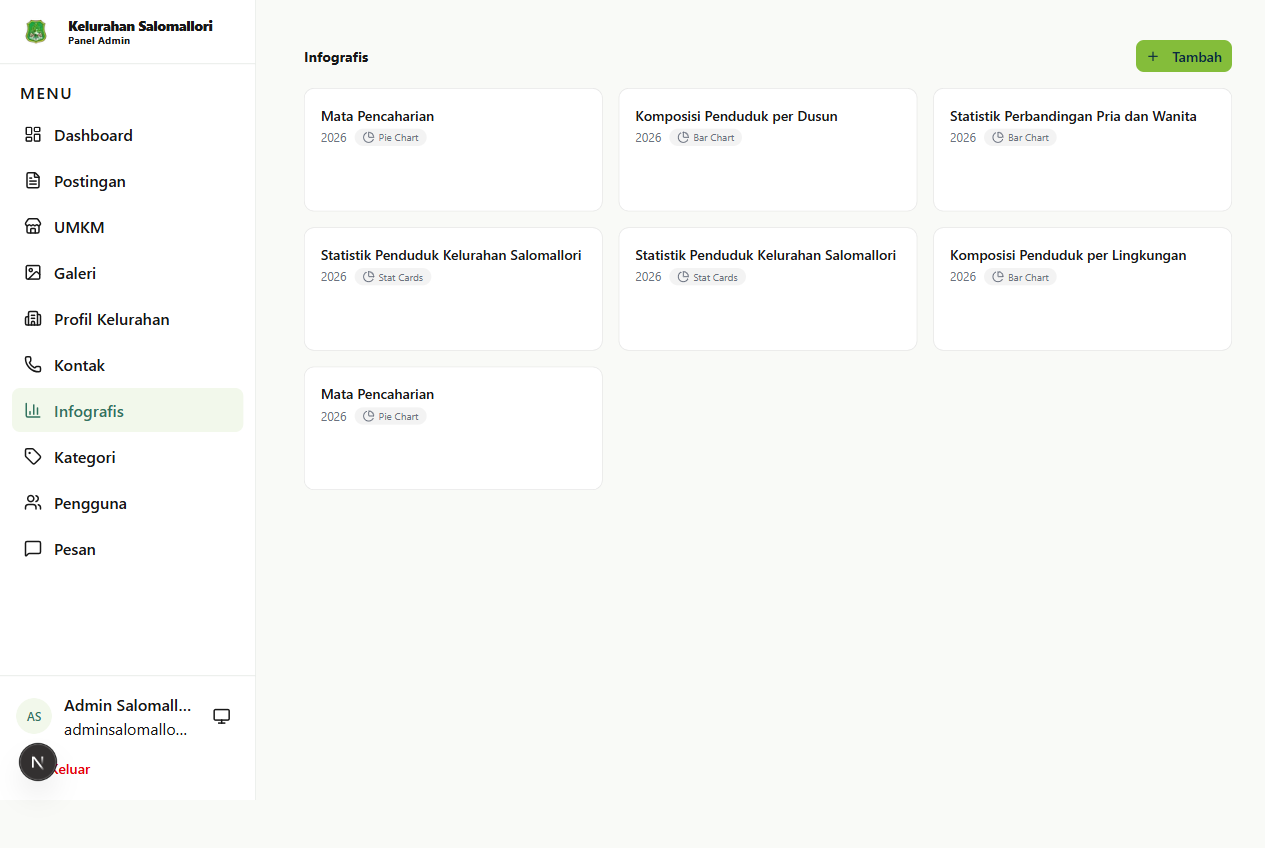
\includegraphics[width=0.85\textwidth]{images/admin-infografis.png}
    \caption{Halaman Kelola Infografis \& Data Statistik}
    \label{fig:admin-infografis}
\end{figure}

\subsection{Mengelola Kontak \& Pesan Masuk (Khusus Admin)}

\subsubsection{Mengelola Kontak}

Langkah-langkah memperbarui informasi kontak:
\begin{enumerate}[leftmargin=2em, itemsep=2pt]
    \item Pilih menu \textbf{Kontak} pada sidebar dashboard;
    \item Perbarui informasi yang tersimpan, antara lain:
    \begin{itemize}[leftmargin=2em, itemsep=2pt]
        \item Alamat kantor kelurahan;
        \item Nomor telepon;
        \item Nomor WhatsApp;
        \item Alamat email;
        \item Jam operasional;
        \item \emph{Maps embed} Google Maps.
    \end{itemize}
    \item Klik \textbf{Simpan}; informasi akan diperbarui di halaman Kontak dan \emph{footer} website.
\end{enumerate}

\begin{figure}[H]
    \centering
    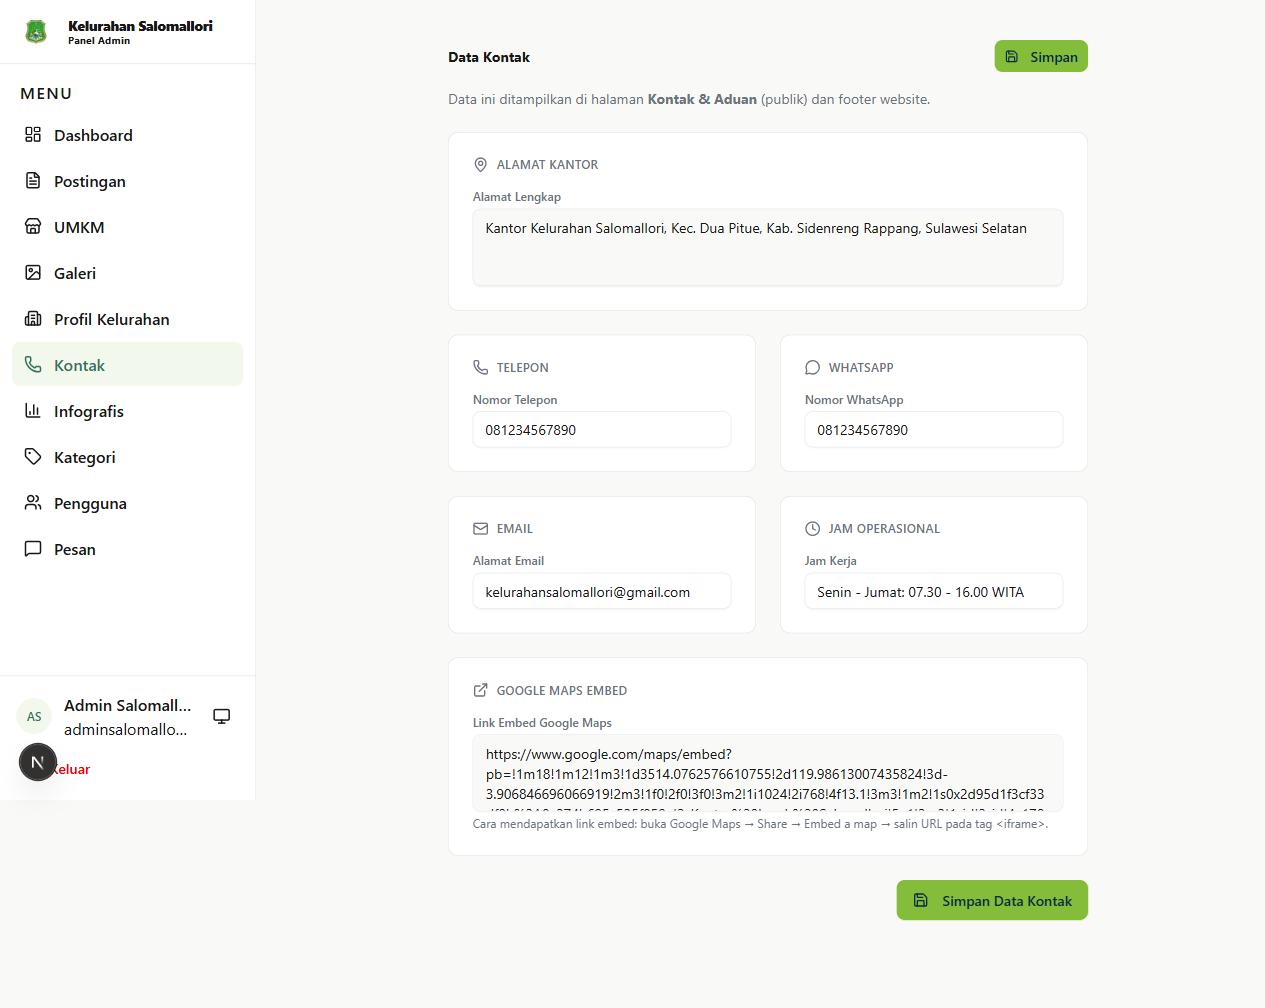
\includegraphics[width=0.85\textwidth]{images/admin-kontak.png}
    \caption{Halaman Kelola Kontak \& Lokasi}
    \label{fig:admin-kontak}
\end{figure}

\subsubsection{Melihat Pesan Masuk}

Langkah-langkah melihat pesan dari pengunjung:
\begin{enumerate}[leftmargin=2em, itemsep=2pt]
    \item Pilih menu \textbf{Pesan} pada sidebar dashboard;
    \item Halaman menampilkan daftar pesan yang berisi \textbf{Pengirim}, \textbf{Email}, \textbf{Isi Pesan}, \textbf{Status} (Baru/Dibaca), dan \textbf{Tanggal};
    \item Klik pesan untuk membaca dan menandai statusnya.
\end{enumerate}

\begin{figure}[H]
    \centering
    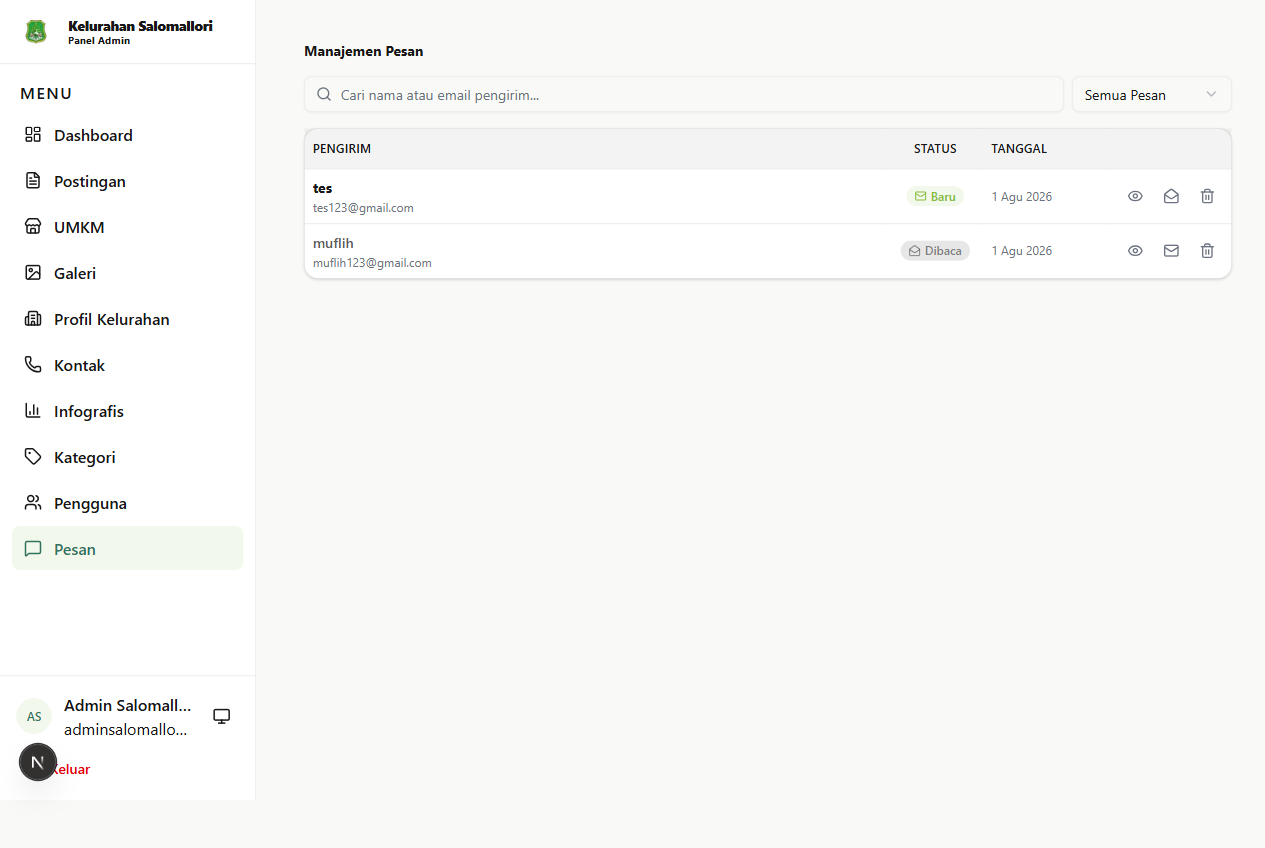
\includegraphics[width=0.85\textwidth]{images/admin-messages.png}
    \caption{Halaman Kotak Masuk Pesan dari Pengunjung}
    \label{fig:admin-messages}
\end{figure}

% ============================================================
% BAB 5: STUDI KASUS / CONTOH PRAKTIK
% ============================================================
\chapter{STUDI KASUS / CONTOH PRAKTIK}

\section{Studi Kasus 1: Penelusuran Visualisasi Infografis Statistik Kependudukan}

\paragraph{Skenario:}
Seorang warga Kelurahan Salomallori ingin melihat data statistik kependudukan kelurahan secara visual.

\paragraph{Langkah Penyelesaian:}
\begin{enumerate}[leftmargin=2em, itemsep=2pt]
    \item Buka \url{https://www.salomallori.web.id} pada browser;
    \item Arahkan kursor ke menu \textbf{Profil} pada navigasi \emph{floating pill};
    \item Pilih sub-menu \textbf{Infografis};
    \item Halaman Infografis menampilkan berbagai visualisasi data statistik (misalnya jumlah penduduk, jumlah KK, atau komposisi penduduk) dalam bentuk \emph{bar chart}, \emph{line chart}, \emph{pie chart}, \emph{doughnut chart}, \emph{area chart}, atau \emph{stat cards};
    \item Warga dapat membaca dan memahami data kelurahan melalui grafik yang tersaji secara visual tanpa perlu mengolah data mentah.
\end{enumerate}

Contoh struktur \emph{dataJson} yang digunakan pada infografis ditunjukkan pada Tabel~\ref{tab:datajson}.

\begin{table}[H]
    \centering
    \caption{Contoh Struktur \texttt{dataJson} pada Infografis}
    \label{tab:datajson}
    \begin{tabularx}{\textwidth}{X X X}
        \toprule
        \textbf{Kunci} & \textbf{Tipe} & \textbf{Keterangan} \\
        \midrule
        \texttt{labels} & Array of String & Label sumbu kategori (misal: nama lingkungan) \\
        \texttt{datasets} & Array of Object & Kumpulan data yang divisualisasikan \\
        \texttt{datasets[].label} & String & Nama seri data (misal: Jumlah Penduduk) \\
        \texttt{datasets[].data} & Array of Number & Nilai numerik yang ditampilkan \\
        \texttt{datasets[].backgroundColor} & Array of String & Warna batang/area (mengacu palet resmi) \\
        \bottomrule
    \end{tabularx}
\end{table}

\begin{figure}[H]
    \centering
    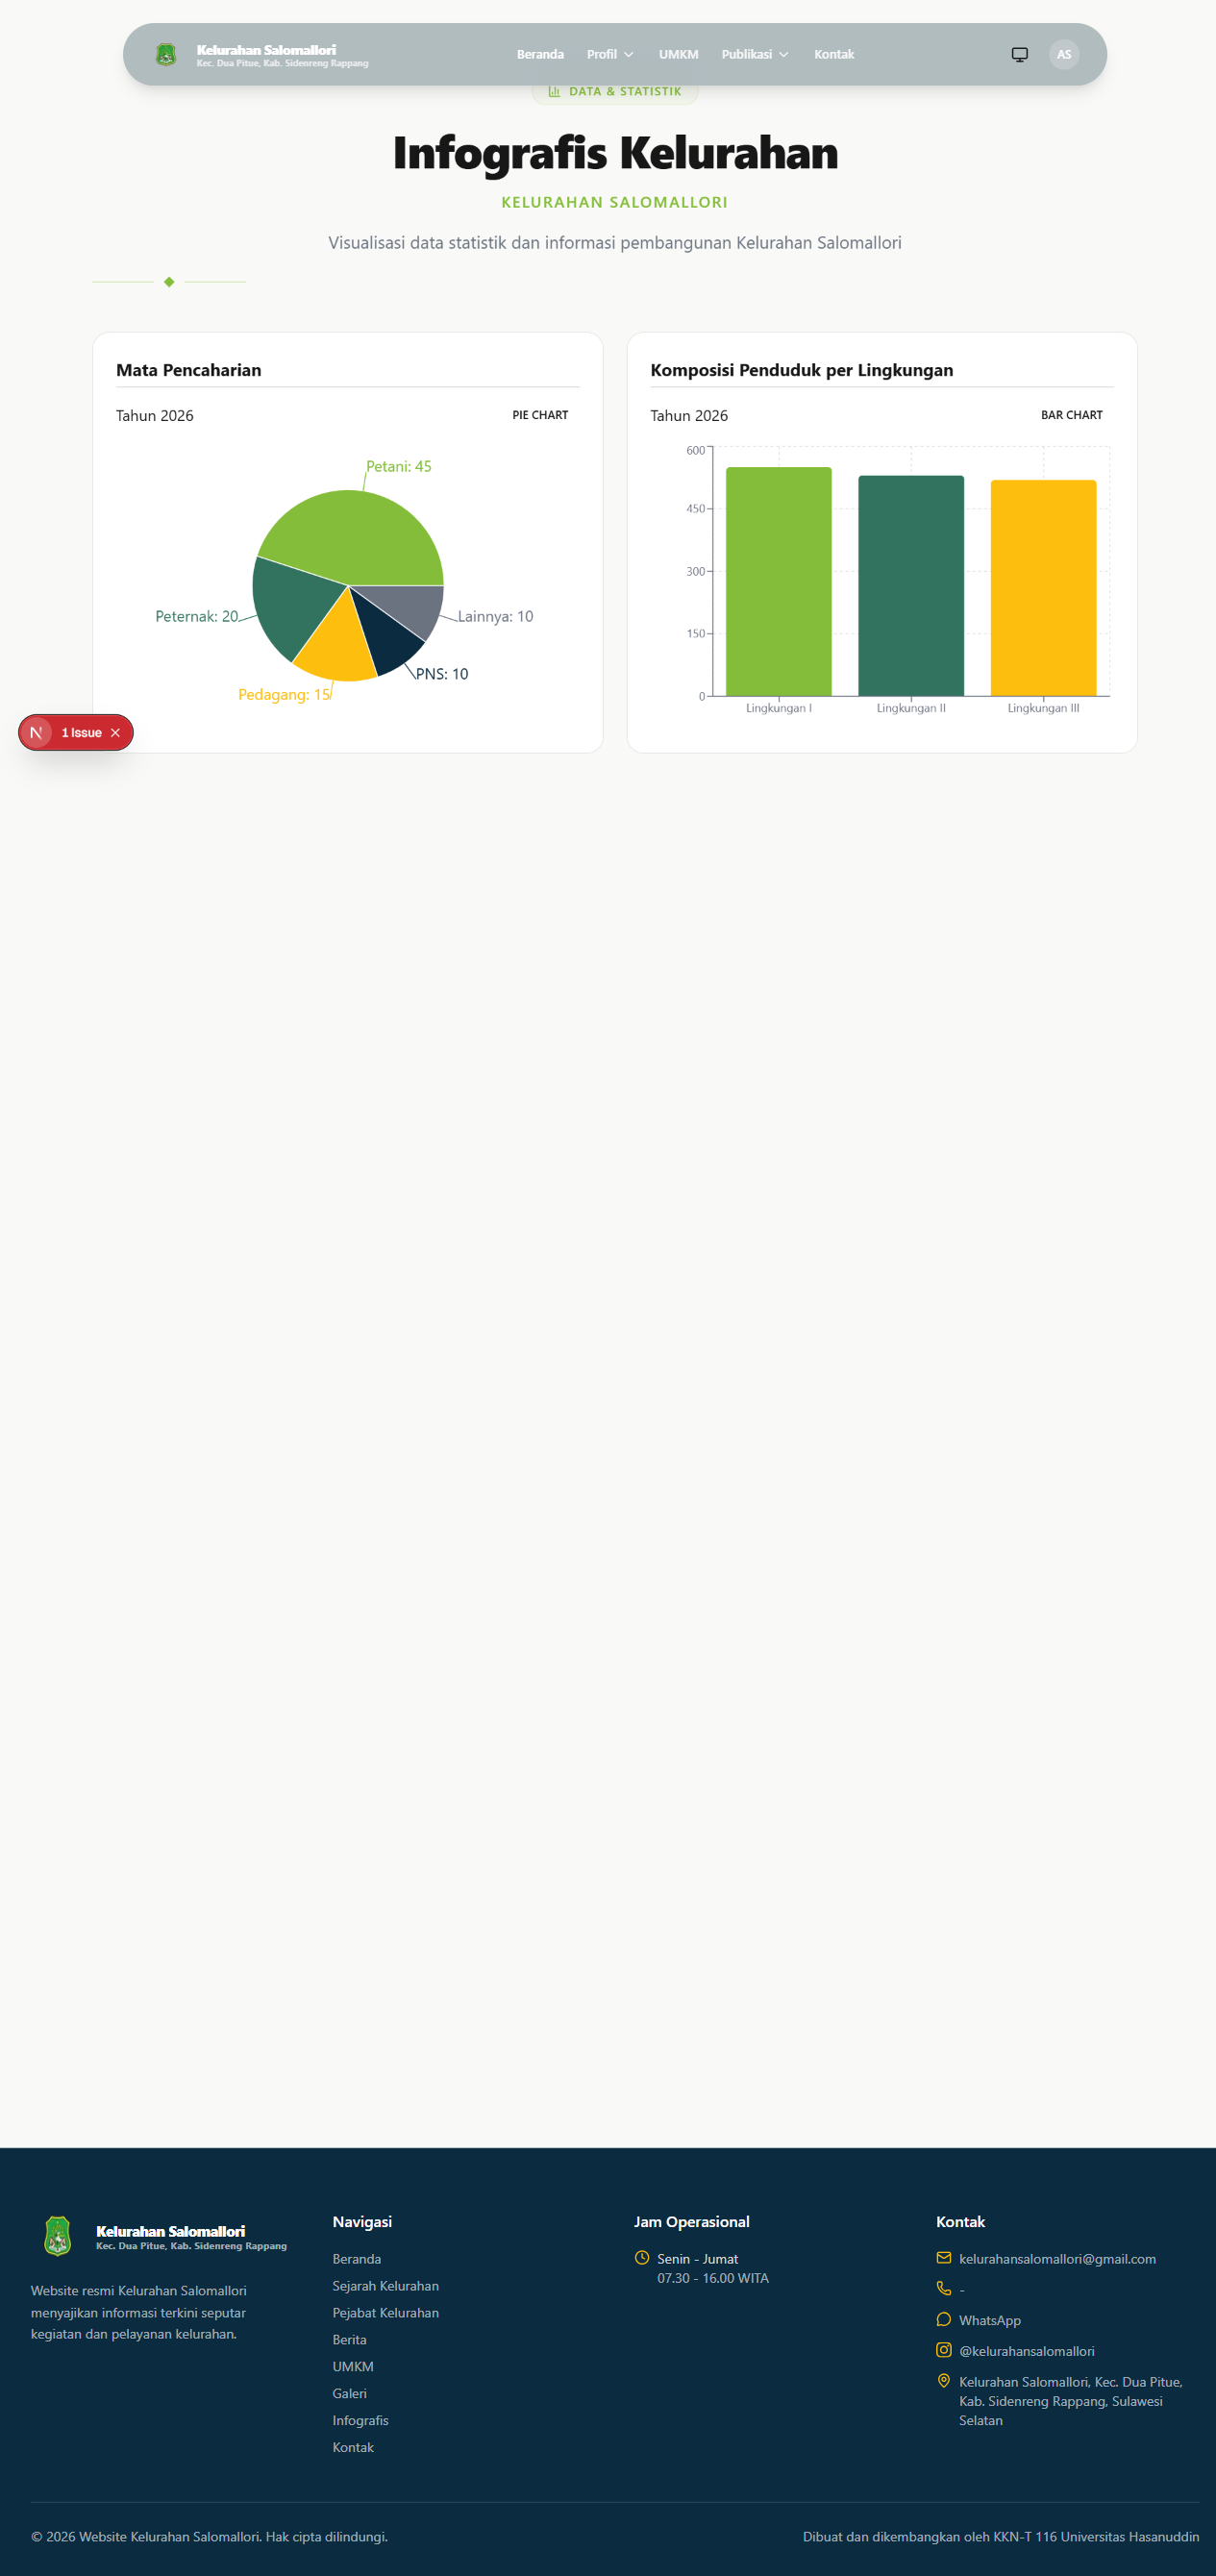
\includegraphics[width=0.85\textwidth]{images/infografis.png}
    \caption{Hasil Akhir: Visualisasi Infografis Statistik pada Halaman Publik}
    \label{fig:kasus1}
\end{figure}

\section{Studi Kasus 2: Penulisan dan Pemublikasian Artikel Kabar Desa Menggunakan TipTap Editor}

\paragraph{Skenario:}
Seorang Editor (perangkat kelurahan) ingin menulis dan mempublikasikan artikel berita tentang kegiatan KKN di Kelurahan Salomallori.

\paragraph{Langkah Penyelesaian:}
\begin{enumerate}[leftmargin=2em, itemsep=2pt]
    \item Login ke dashboard melalui halaman \texttt{/auth/signin};
    \item Pilih menu \textbf{Postingan} pada sidebar;
    \item Klik \textbf{Buat Postingan};
    \item Isi \textbf{Judul} artikel, misalnya \emph{``Mahasiswa KKN Unhas Menyelenggarakan Sosialisasi Digitalisasi Kelurahan''};
    \item Tulis \textbf{Konten} menggunakan \textbf{TipTap Rich Text Editor}:
    \begin{itemize}[leftmargin=2em, itemsep=2pt]
        \item Gunakan tombol \textbf{Bold} dan \textbf{Italic} untuk menegaskan kata penting;
        \item Gunakan \textbf{Heading} untuk membagi sub-bagian artikel;
        \item Gunakan \textbf{Bullet List} atau \textbf{Numbered List} untuk rincian;
        \item Sisipkan \textbf{Link} jika merujuk pada sumber eksternal;
        \item Sisipkan \textbf{Gambar} untuk memperkaya artikel.
    \end{itemize}
    \item Pilih \textbf{Kategori} artikel;
    \item Unggah \textbf{Gambar Sampul} melalui fitur \emph{upload};
    \item Klik \textbf{Terbitkan};
    \item Verifikasi artikel telah tampil di halaman Berita (\texttt{/news}) pada situs publik.
\end{enumerate}

\begin{figure}[H]
    \centering
    \begin{subfigure}{0.45\textwidth}
        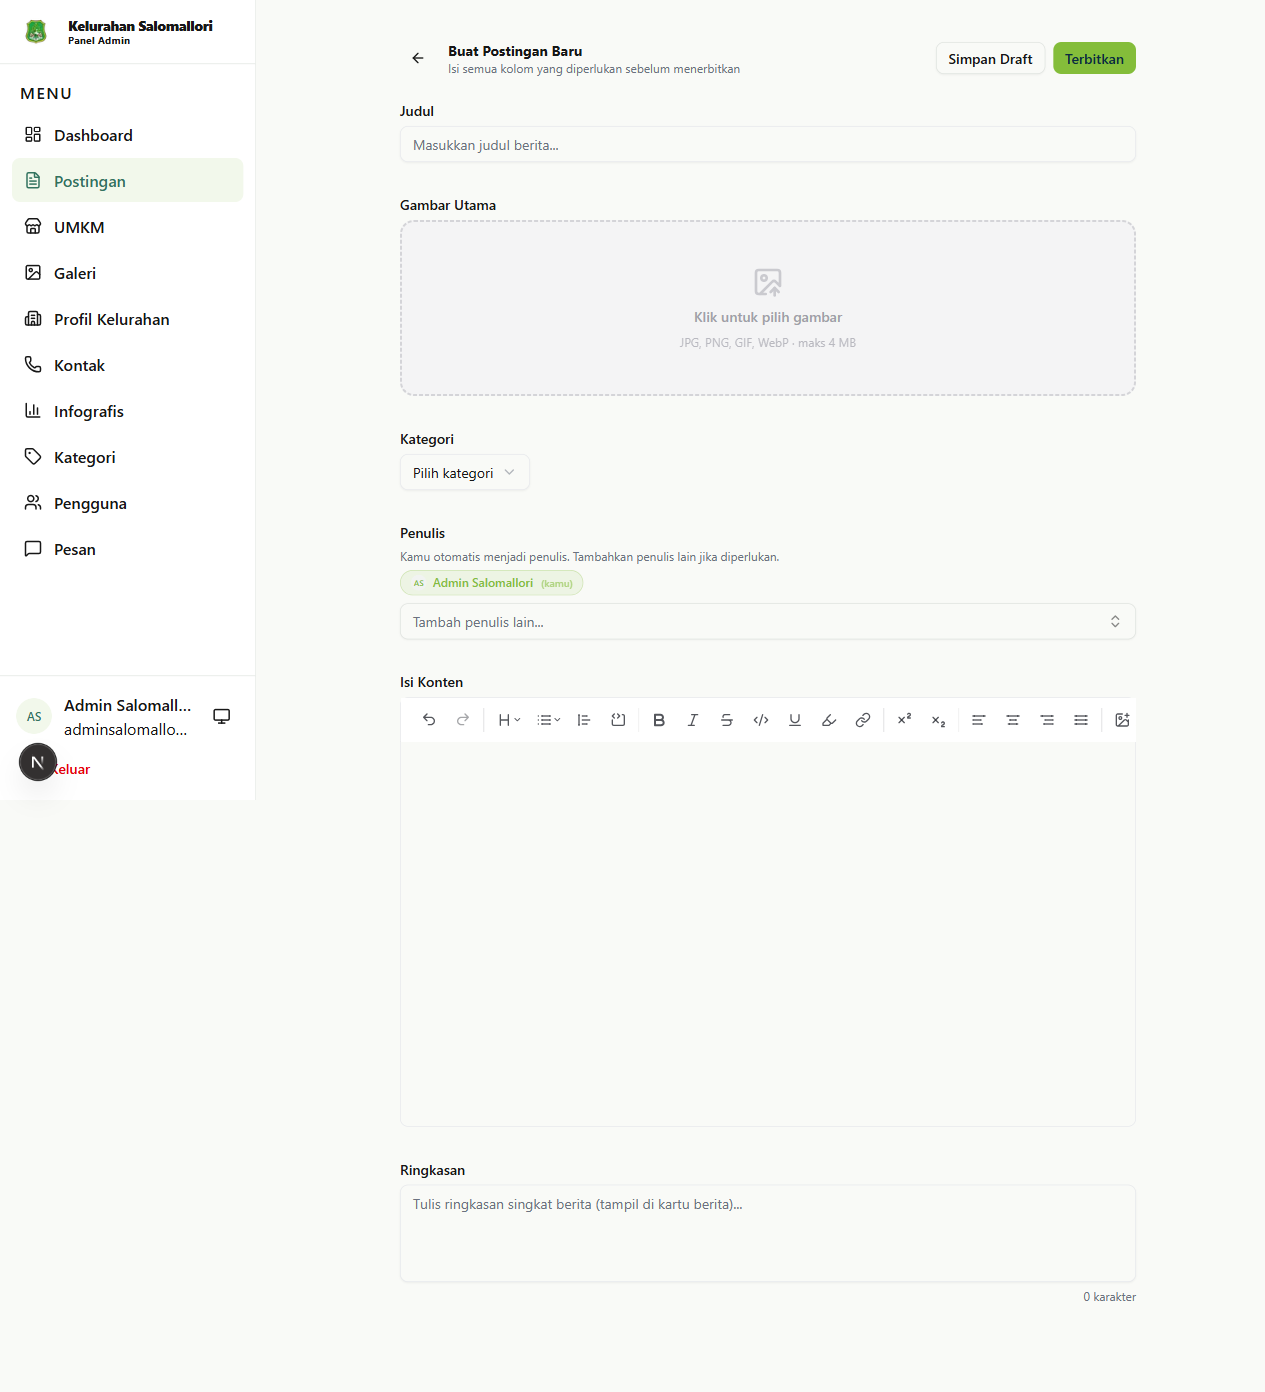
\includegraphics[width=\textwidth]{images/admin-posts-create.png}
        \caption{Form Penulisan dengan TipTap Editor}
    \end{subfigure}
    \hfill
    \begin{subfigure}{0.45\textwidth}
        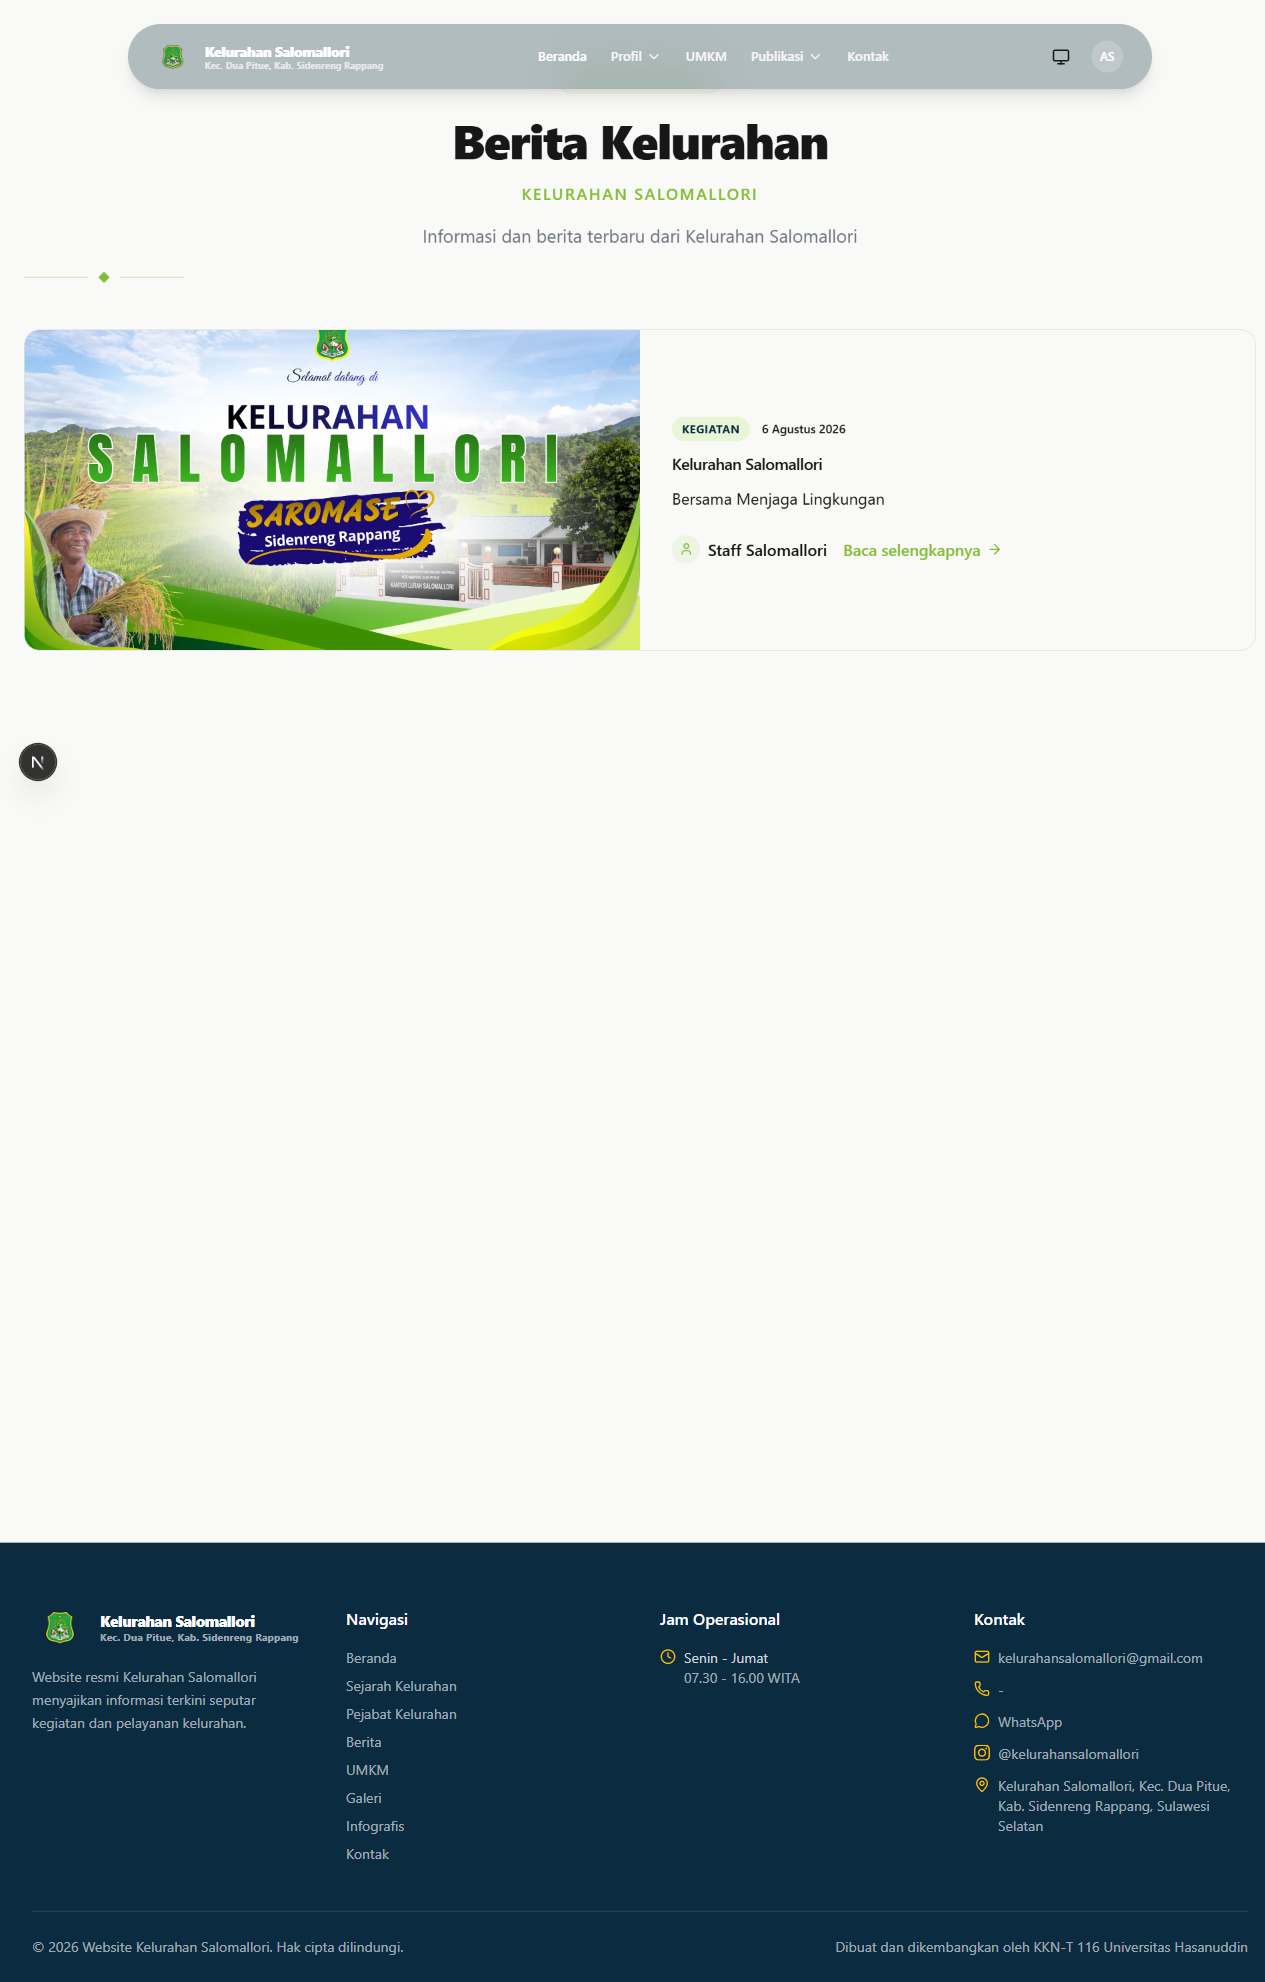
\includegraphics[width=\textwidth]{images/berita.png}
        \caption{Artikel Terbit di Halaman Berita Publik}
    \end{subfigure}
    \caption{Studi Kasus 2: Penulisan dan Pemublikasian Artikel}
    \label{fig:kasus2}
\end{figure}

\section{Studi Kasus 3: Penambahan Katalog Produk UMKM Lokal beserta Foto Produk oleh Editor}

\paragraph{Skenario:}
Seorang Editor ingin menambahkan produk UMKM warga ke dalam katalog website.

\paragraph{Langkah Penyelesaian:}
\begin{enumerate}[leftmargin=2em, itemsep=2pt]
    \item Login ke dashboard;
    \item Pilih menu \textbf{UMKM} pada sidebar;
    \item Klik \textbf{Tambah UMKM};
    \item Lengkapi formulir, yaitu:
    \begin{itemize}[leftmargin=2em, itemsep=2pt]
        \item \textbf{Nama Produk}: misal \emph{``Telur Ayam Ras Fresh''};
        \item \textbf{Deskripsi}: uraian singkat produk;
        \item \textbf{Harga}: harga jual produk;
        \item \textbf{Kategori}: pilih kategori yang sesuai;
        \item \textbf{Pemilik}: nama pemilik usaha;
        \item \textbf{Kontak}: nomor yang dapat dihubungi.
    \end{itemize}
    \item Unggah \textbf{Gambar Produk} melalui fitur \emph{upload} Cloudinary;
    \item Klik \textbf{Simpan};
    \item Verifikasi produk telah tampil pada halaman Katalog UMKM (\texttt{/umkm}) di situs publik.
\end{enumerate}

\begin{figure}[H]
    \centering
    \begin{subfigure}{0.45\textwidth}
        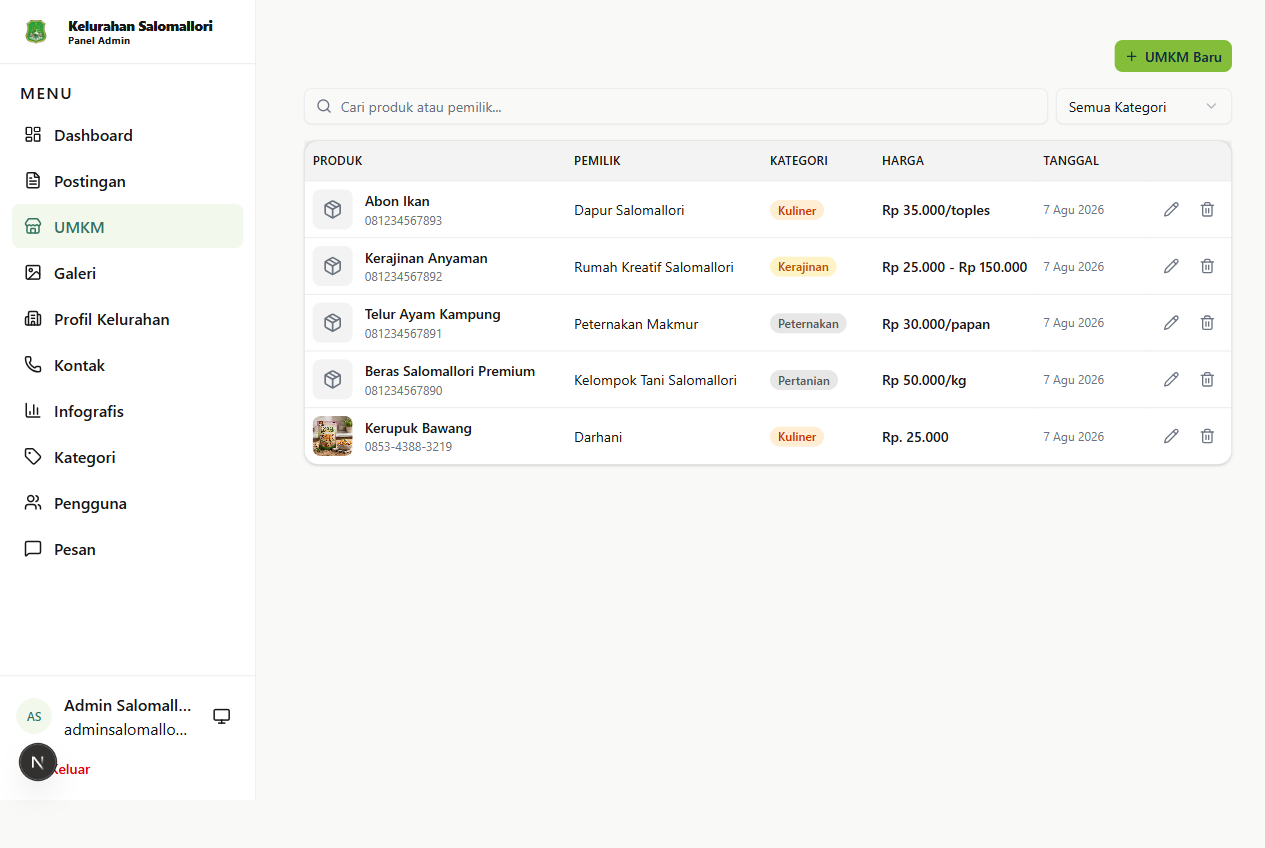
\includegraphics[width=\textwidth]{images/admin-umkm.png}
        \caption{Daftar Kelola UMKM pada Dashboard}
    \end{subfigure}
    \hfill
    \begin{subfigure}{0.45\textwidth}
        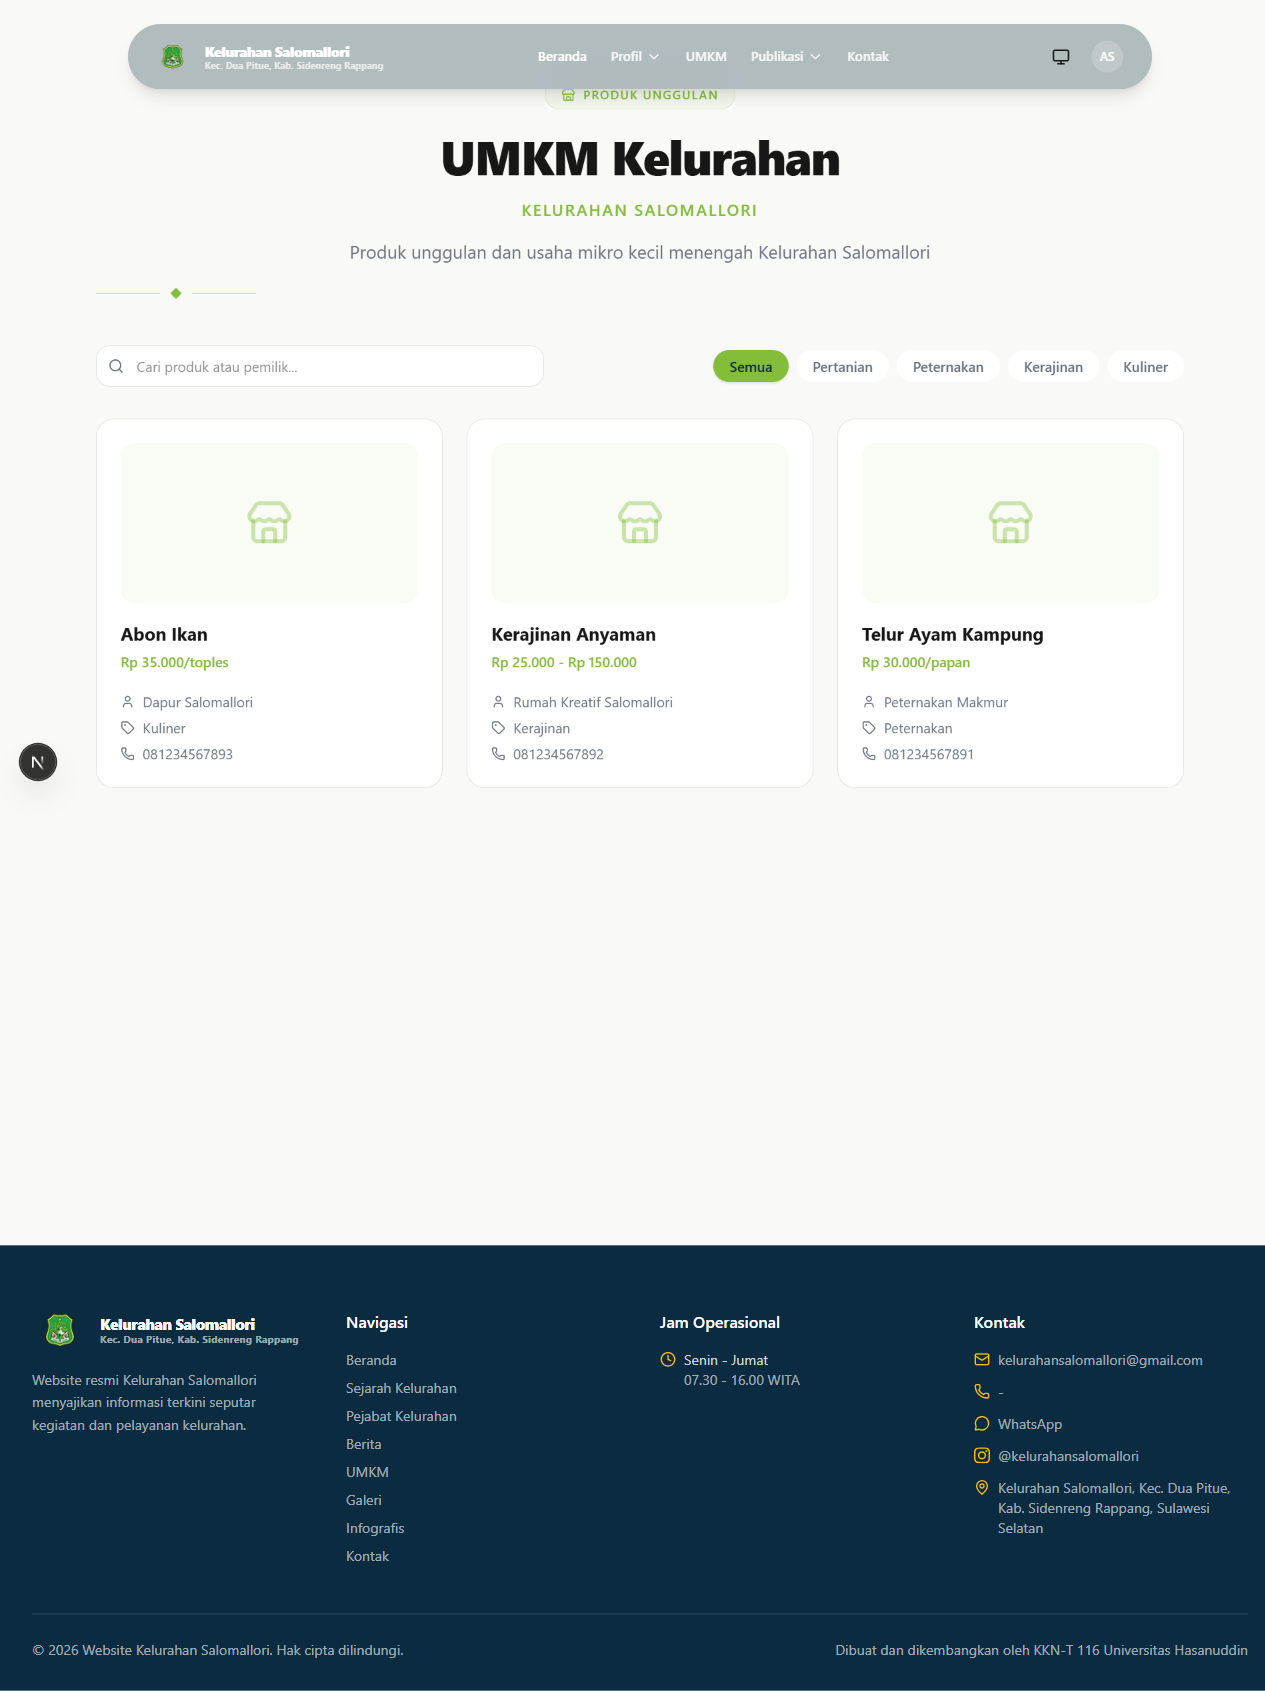
\includegraphics[width=\textwidth]{images/umkm.png}
        \caption{Produk UMKM Tampil di Halaman Publik}
    \end{subfigure}
    \caption{Studi Kasus 3: Penambahan Katalog Produk UMKM}
    \label{fig:kasus3}
\end{figure}

\section{Studi Kasus 4: Pembaruan Data Demografi pada Halaman Pendataan oleh Administrator}

\paragraph{Skenario:}
Seorang Administrator ingin memperbarui data demografi kelurahan, misalnya mengubah jumlah kepala keluarga menjadi 1.077 KK atau memperbarui batas wilayah kelurahan.

\paragraph{Langkah Penyelesaian:}
\begin{enumerate}[leftmargin=2em, itemsep=2pt]
    \item Login ke dashboard menggunakan akun Administrator;
    \item Pilih menu \textbf{Profil Kelurahan} pada sidebar dashboard;
    \item Lakukan pembaruan pada \textbf{Halaman Pendataan}, antara lain:
    \begin{itemize}[leftmargin=2em, itemsep=2pt]
        \item Perbarui \textbf{Luas Wilayah} (misal: \emph{7,63 km²});
        \item Perbarui \textbf{Jumlah Penduduk} (misal: \emph{3.234 jiwa});
        \item Perbarui \textbf{Jumlah Kepala Keluarga} (misal: \emph{1.077 KK});
        \item Perbarui \textbf{Jumlah Lingkungan} (misal: \emph{3 lingkungan});
        \item Perbarui \textbf{Batas Wilayah} (Utara, Timur, Selatan, Barat);
        \item Perbarui \textbf{Sejarah}, \textbf{Visi}, dan \textbf{Misi} kelurahan jika diperlukan.
    \end{itemize}
    \item Klik \textbf{Simpan} untuk menyimpan perubahan;
    \item Verifikasi data baru telah tampil pada halaman publik, yaitu di Beranda (ringkasan statistik) dan halaman Sejarah Kelurahan.
\end{enumerate}

\begin{figure}[H]
    \centering
    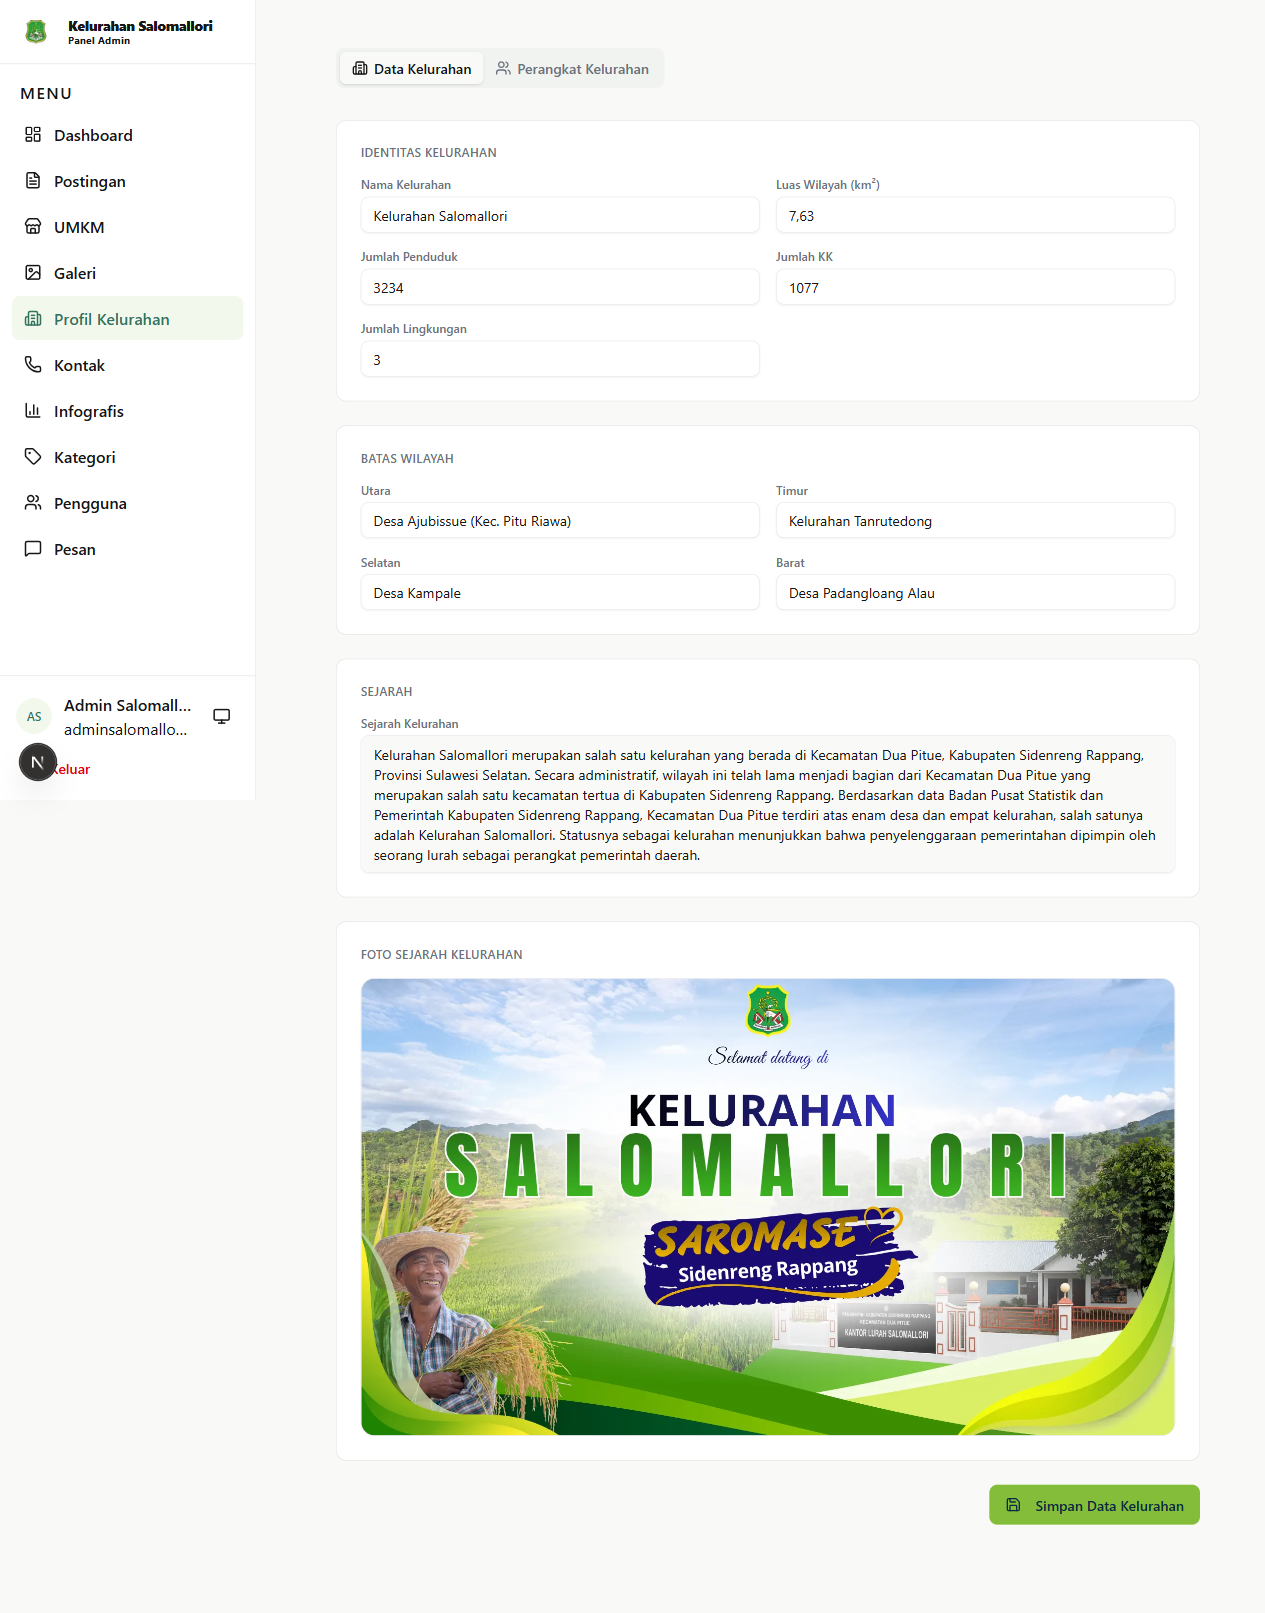
\includegraphics[width=0.85\textwidth]{images/admin-profil-desa.png}
    \caption{Studi Kasus 4: Pembaruan Data Demografi pada Halaman Pendataan}
    \label{fig:kasus4}
\end{figure}

% ============================================================
% BAB 6: PENUTUP
% ============================================================
\chapter{PENUTUP}

\section{Kesimpulan}

Website Profil Kelurahan Salomallori merupakan wujud nyata pemanfaatan teknologi informasi untuk memperkuat tata kelola informasi publik di tingkat kelurahan. Melalui platform yang dibangun dengan arsitektur web modern (Next.js 16, React 19, Tailwind CSS 4, PostgreSQL, dan Prisma ORM), kelurahan memiliki:

\begin{enumerate}[leftmargin=2em, itemsep=2pt]
    \item \textbf{Portal informasi terpadu} yang menyajikan profil kelurahan, kabar desa, katalog UMKM, galeri foto, dan visualisasi data statistik dalam satu tempat;
    \item \textbf{Sistem pengelolaan konten yang mudah digunakan} oleh perangkat kelurahan melalui dashboard administrator dan editor, lengkap dengan editor teks kaya (TipTap) dan pengunggah gambar (Cloudinary);
    \item \textbf{Sistem pembagian hak akses yang jelas} (\emph{Role-Based Access Control}) untuk level USER, EDITOR, dan ADMIN sehingga keamanan dan keabsahan data tetap terjaga;
    \item \textbf{Tampilan yang modern dan responsif} dengan palet warna resmi kelurahan serta dukungan mode terang dan gelap.
\end{enumerate}

Ketersediaan buku panduan ini diharapkan dapat menjembatani seluruh pengguna, baik masyarakat umum maupun pengelola sistem, untuk memanfaatkan website secara optimal sehingga transparansi informasi dan promosi potensi kelurahan dapat berjalan secara berkelanjutan.

\section{Saran \& Rekomendasi Pemeliharaan}

Agar website tetap relevan, aktual, dan aman, disarankan beberapa hal berikut:

\begin{enumerate}[leftmargin=2em, itemsep=2pt]
    \item \textbf{Pembaruan data secara berkala}:
    \begin{itemize}[leftmargin=2em, itemsep=2pt]
        \item Melakukan pembaruan data statistik pada beranda (jumlah jiwa, luas wilayah) dan artikel berita kelurahan secara berkala;
        \item Memperbarui data profil kelurahan, perangkat, dan infografis setiap ada perubahan.
    \end{itemize}
    \item \textbf{Manajemen keamanan}:
    \begin{itemize}[leftmargin=2em, itemsep=2pt]
        \item Melakukan manajemen pengaturan kata sandi dan kontrol keamanan \emph{Role-Based Access} (USER, ADMIN, EDITOR) dengan ketat;
        \item Menjaga kerahasiaan kredensial akun administrator dan editor.
    \end{itemize}
    \item \textbf{Pengelolaan media}:
    \begin{itemize}[leftmargin=2em, itemsep=2pt]
        \item Mengevaluasi batas kuota penyimpanan media gambar pada layanan \emph{Cloudinary};
        \item Melakukan pembersihan file media yang tidak terpakai secara berkala.
    \end{itemize}
    \item \textbf{Pengembangan lanjutan}: Menindaklanjuti rencana penambahan Peta Interaktif Wilayah (Fase 6) setelah data GeoJSON batas dusun dan titik penting tersedia dari tim GIS.
\end{enumerate}

% ============================================================
% BAGIAN AKHIR
% ============================================================

% ---------- BIBLIOGRAFI / DAFTAR PUSTAKA ----------
\unnumberedchapter{BIBLIOGRAFI / DAFTAR PUSTAKA}

\begin{enumerate}[leftmargin=2em, itemsep=6pt]
    \item Rezky Robby. (2024). \emph{Portal Berita Kodim -- Repositori Basis Kode}. GitHub. \url{https://github.com/RezkyRobby23h/PortalBeritaKodim}
    \item Vercel. (2026). \emph{Next.js Documentation: App Router}. \url{https://nextjs.org/docs}
    \item Prisma. (2026). \emph{Prisma ORM Documentation}. \url{https://www.prisma.io/docs}
    \item Tailwind CSS. (2026). \emph{Tailwind CSS Documentation}. \url{https://tailwindcss.com/docs}
    \item Better Auth. (2026). \emph{Better Auth Documentation}. \url{https://www.better-auth.com}
    \item TipTap. (2026). \emph{TipTap Editor Documentation}. \url{https://tiptap.dev}
    \item Cloudinary. (2026). \emph{Cloudinary Documentation}. \url{https://cloudinary.com/documentation}
    \item Google. (2026). \emph{Google Maps Embed API Documentation}. \url{https://developers.google.com/maps/documentation/embed}
    \item Recharts. (2026). \emph{Recharts Documentation}. \url{https://recharts.org}
    \item shadcn/ui. (2026). \emph{shadcn/ui Documentation}. \url{https://ui.shadcn.com}
    \item Badan Pusat Statistik. (2026). \emph{Data Demografi Kelurahan Salomallori, Kecamatan Dua Pitue, Kabupaten Sidenreng Rappang}.
\end{enumerate}

\clearpage

% ---------- LAMPIRAN ----------
\appendix

\chapter{LAMPIRAN A: PETA \emph{ROUTE MAPPING} SELURUH HALAMAN WEBSITE PUBLIK \& DASBOR ADMIN}

Berikut adalah peta seluruh rute (route mapping) halaman pada website, baik untuk pengguna publik maupun pengelola (dashboard admin).

\section*{A.1 Halaman Publik}

\begin{longtable}{p{0.08\textwidth} p{0.30\textwidth} p{0.20\textwidth} p{0.34\textwidth}}
    \caption{Rute Halaman Publik}\\
    \toprule
    \textbf{No} & \textbf{Rute} & \textbf{Tipe Halaman} & \textbf{Keterangan} \\
    \midrule
    \endfirsthead
    \toprule
    \textbf{No} & \textbf{Rute} & \textbf{Tipe Halaman} & \textbf{Keterangan} \\
    \midrule
    \endhead
    \bottomrule
    \endfoot
    1 & \texttt{/} & Beranda & Hero, statistik, berita, sejarah, galeri \\
    2 & \texttt{/profil} & Profil & Profil kelurahan (data Desa) \\
    3 & \texttt{/profil/sejarah-kelurahan} & Sejarah & Sejarah kelurahan \\
    4 & \texttt{/profil/pejabat-kelurahan} & Pejabat & Pejabat kelurahan \\
    5 & \texttt{/profil/visi-misi} & Visi Misi & Visi dan misi \\
    6 & \texttt{/profil/struktur-organisasi} & Struktur & Bagan struktur organisasi \\
    7 & \texttt{/news} & Berita & Daftar berita \\
    8 & \texttt{/news/[slug]} & Berita & Detail artikel berita \\
    9 & \texttt{/umkm} & UMKM & Katalog produk UMKM \\
    10 & \texttt{/umkm/[id]} & UMKM & Detail produk UMKM \\
    11 & \texttt{/wisata} & Wisata & Daftar wisata \\
    12 & \texttt{/wisata/[id]} & Wisata & Detail destinasi wisata \\
    13 & \texttt{/galeri} & Galeri & Galeri foto + lightbox \\
    14 & \texttt{/infografis} & Infografis & Visualisasi data statistik \\
    15 & \texttt{/kontak} & Kontak & Kontak + Google Maps \\
    \end{longtable}

\section*{A.2 Halaman Autentikasi \& Akun}

\begin{longtable}{p{0.08\textwidth} p{0.30\textwidth} p{0.20\textwidth} p{0.34\textwidth}}
    \caption{Rute Autentikasi dan Akun Pengguna}\\
    \toprule
    \textbf{No} & \textbf{Rute} & \textbf{Tipe Halaman} & \textbf{Keterangan} \\
    \midrule
    \endfirsthead
    \toprule
    \textbf{No} & \textbf{Rute} & \textbf{Tipe Halaman} & \textbf{Keterangan} \\
    \midrule
    \endhead
    \bottomrule
    \endfoot
    1 & \texttt{/auth/signin} & Autentikasi & Halaman masuk (login) \\
    2 & \texttt{/auth/signup} & Autentikasi & Halaman pendaftaran (register) \\
    3 & \texttt{/akun/[id]} & Akun & Halaman profil pengguna \\
    \end{longtable}

\section*{A.3 Halaman Dashboard Admin}

\begin{longtable}{p{0.08\textwidth} p{0.30\textwidth} p{0.20\textwidth} p{0.34\textwidth}}
    \caption{Rute Dashboard Administrator dan Editor}\\
    \toprule
    \textbf{No} & \textbf{Rute} & \textbf{Tipe Halaman} & \textbf{Keterangan} \\
    \midrule
    \endfirsthead
    \toprule
    \textbf{No} & \textbf{Rute} & \textbf{Tipe Halaman} & \textbf{Keterangan} \\
    \midrule
    \endhead
    \bottomrule
    \endfoot
    1 & \texttt{/dashboard} & Overview & Ringkasan analitik portal \\
    2 & \texttt{/dashboard/posts} & Postingan & CRUD berita \\
    3 & \texttt{/dashboard/posts/create} & Postingan & Form berita baru \\
    4 & \texttt{/dashboard/posts/[id]} & Postingan & Edit berita \\
    5 & \texttt{/dashboard/umkm} & UMKM & CRUD UMKM \\
    6 & \texttt{/dashboard/umkm/new} & UMKM & Form UMKM baru \\
    7 & \texttt{/dashboard/umkm/[id]/edit} & UMKM & Edit UMKM \\
    8 & \texttt{/dashboard/wisata} & Wisata & CRUD wisata \\
    9 & \texttt{/dashboard/wisata/new} & Wisata & Form wisata baru \\
    10 & \texttt{/dashboard/wisata/[id]/edit} & Wisata & Edit wisata \\
    11 & \texttt{/dashboard/galeri} & Galeri & Kelola galeri foto \\
    12 & \texttt{/dashboard/profil-desa} & Profil Desa & Edit profil kelurahan \& perangkat \\
    13 & \texttt{/dashboard/infografis} & Infografis & Kelola infografis \\
    14 & \texttt{/dashboard/kontak} & Kontak & Kelola kontak \& lokasi \\
    15 & \texttt{/dashboard/messages} & Pesan & Kelola pesan masuk \\
    16 & \texttt{/dashboard/categories} & Kategori & CRUD kategori \\
    17 & \texttt{/dashboard/users} & Pengguna & Manajemen pengguna (admin only) \\
    \end{longtable}

\clearpage

\chapter{LAMPIRAN B: KAMUS DATA / SKEMA DATABASE PRISMA}

Kamus data berikut merangkum model-model utama pada skema database Prisma yang digunakan oleh website.

\begin{longtable}{p{0.22\textwidth} p{0.14\textwidth} p{0.56\textwidth}}
    \caption{Kamus Data Model Utama Prisma}\\
    \toprule
    \textbf{Model} & \textbf{Tabel} & \textbf{Bidang Utama} \\
    \midrule
    \endfirsthead
    \toprule
    \textbf{Model} & \textbf{Tabel} & \textbf{Bidang Utama} \\
    \midrule
    \endhead
    \bottomrule
    \endfoot
    \texttt{User} & \texttt{user} & id, name, email, role (USER/EDITOR/ADMIN) \\
    \texttt{Post} & \texttt{post} & id, judul, slug, konten, gambar, categoryId, trending, isHighlight, published \\
    \texttt{Category} & \texttt{category} & id, nama, slug \\
    \texttt{BreakingNews} & \texttt{breaking\_news} & id, konten, aktif \\
    \texttt{Message} & \texttt{message} & id, nama, email, pesan, status \\
    \texttt{Desa} & \texttt{desa} & id, nama, sejarah, visi, misi, luasWilayah, jumlahPenduduk, jumlahKK, jumlahDusun, batasUtara, batasTimur, batasSelatan, batasBarat, fotoKepalaDesa \\
    \texttt{PerangkatDesa} & \texttt{perangkat\_desa} & id, nama, jabatan, foto, urutan \\
    \texttt{UMKM} & \texttt{umkm} & id, namaProduk, deskripsi, harga, kategori, kontak, gambar, pemilik \\
    \texttt{Wisata} & \texttt{wisata} & id, nama, deskripsi, lokasi, kategori (WISATA\_ALAM/KULINER/BUDAYA), gambar \\
    \texttt{Galeri} & \texttt{galeri} & id, judul, gambar, kategori, uploadedById \\
    \texttt{Infografis} & \texttt{infografis} & id, judul, tahun, dataJson, chartType \\
    \texttt{Kontak} & \texttt{kontak} & id, alamat, telepon, whatsapp, email, jamKerja, mapsEmbed \\
    \end{longtable}

\clearpage

\chapter{LAMPIRAN C: PANDUAN DESAIN SISTEM}

Lampiran ini merangkum panduan desain sistem resmi Kelurahan Salomallori.

\section*{C.1 Palet Warna Resmi}

\begin{table}[H]
    \centering
    \caption{Palet Warna Resmi Kelurahan Salomallori}
    \label{tab:palet}
    \begin{tabularx}{\textwidth}{l l X}
        \toprule
        \textbf{Nama Warna} & \textbf{Hex} & \textbf{Penggunaan} \\
        \midrule
        \textcolor{primarygreen}{\textbf{Primary Green}} & \texttt{\#84BD3A} & Tombol, tautan, state aktif, chart utama \\
        \textcolor{tealdark}{\textbf{Teal Dark}} & \texttt{\#32735F} & Aksen profil, border mode gelap, hover mode gelap \\
        \textcolor{midnight}{\textbf{Midnight Blue}} & \texttt{\#0B2B40} & Navbar, footer, latar mode gelap \\
        \textcolor{gold}{\textbf{Gold}} & \texttt{\#FEBE0D} & Aksen emas, highlight, badge \\
        \textcolor{linen}{\textbf{Linen}} & \texttt{\#F9FAF7} & Latar utama mode terang \\
        \textcolor{sage}{\textbf{Sage}} & \texttt{\#DEE2DE} & Border, outline, pembatas \\
        \textcolor{iron}{\textbf{Iron}} & \texttt{\#6B7280} & Teks sekunder, keterangan \\
        \textcolor{obsidian}{\textbf{Obsidian}} & \texttt{\#171717} & Judul, teks utama mode terang \\
        \bottomrule
    \end{tabularx}
\end{table}

\section*{C.2 Tipografi}

\begin{table}[H]
    \centering
    \caption{Tipografi Font Resmi}
    \label{tab:tipografi}
    \begin{tabularx}{\textwidth}{l X}
        \toprule
        \textbf{Font} & \textbf{Penggunaan} \\
        \midrule
        Montserrat & Font display / heading (judul \& sub-judul) \\
        Geist & Font body / antarmuka (teks isi \& komponen UI) \\
        Geist Mono & Font mono / kode (elemen kode, nomor, dll.) \\
        \bottomrule
    \end{tabularx}
\end{table}

\section*{C.3 Gaya Visual}

\begin{itemize}[leftmargin=2em, itemsep=2pt]
    \item \textbf{Editorial-First}: tipografi menjadi elemen visual utama dengan tata letak bersih;
    \item \textbf{Minimalism}: penggunaan ruang putih (white space) yang luas;
    \item \textbf{Glassmorphism}: navbar mengapung dengan efek \emph{backdrop blur};
    \item \textbf{Floating Architecture}: elemen navigasi mengapung (floating pill).
\end{itemize}

\clearpage

\chapter{LAMPIRAN D: GLOSARIUM ISTILAH TEKNIS WEB MODERN}

\renewcommand{\arraystretch}{1.3}
\begin{longtable}{p{0.28\textwidth} p{0.64\textwidth}}
    \caption{Glosarium Istilah Teknis}\\
    \toprule
    \textbf{Istilah} & \textbf{Definisi} \\
    \midrule
    \endfirsthead
    \toprule
    \textbf{Istilah} & \textbf{Definisi} \\
    \midrule
    \endhead
    \bottomrule
    \endfoot
    \textbf{SSR} (Server-Side Rendering) & Teknik merender halaman web di sisi server sehingga konten tampil lebih cepat dan ramah mesin pencari. \\
    \textbf{CRUD} & Singkatan dari \emph{Create, Read, Update, Delete} -- empat operasi dasar pengelolaan data. \\
    \textbf{ORM} (Object-Relational Mapping) & Teknik menghubungkan objek kode program dengan tabel database, contohnya Prisma. \\
    \textbf{Prisma} & ORM modern untuk Node.js dan TypeScript yang memudahkan akses database PostgreSQL. \\
    \textbf{TipTap} & Editor teks kaya (\emph{rich text editor}) berbasis ProseMirror untuk aplikasi web. \\
    \textbf{Cloudinary} & Layanan cloud untuk penyimpanan, pengelolaan, dan optimasi gambar serta media. \\
    \textbf{RBAC} (Role-Based Access Control) & Sistem pengendalian akses yang membagi hak pengguna berdasarkan peran (USER, EDITOR, ADMIN). \\
    \textbf{PostgreSQL} & Sistem manajemen basis data relasional open source. \\
    \textbf{Next.js} & Framework React untuk membangun aplikasi web dengan \emph{App Router} dan SSR. \\
    \textbf{Tailwind CSS} & Kerangka kerja CSS berbasis utility untuk mempercepat pembuatan antarmuka. \\
    \textbf{Better-Auth} & Pustaka autentikasi modern yang menyediakan login, sesi, dan manajemen pengguna. \\
    \textbf{Recharts} & Pustaka grafik untuk React yang digunakan pada halaman Infografis. \\
    \textbf{Glassmorphism} & Gaya desain dengan efek transparan dan \emph{backdrop blur}. \\
    \textbf{Floating Pill} & Bentuk navigasi mengapung dengan sudut membulat penuh (rounded-full). \\
    \textbf{GeoJSON} & Format standar untuk merepresentasikan data geografis (direncanakan untuk Peta Interaktif). \\
    \end{longtable}

\end{document}
